\declarecommand{\libos}{libOS}
\declarecommand{\sysname}{Graphene}
\declarecommand{\pal}{PAL}
\declarecommand{\syscalls}{131}
\declarecommand{\palcalls}{43}
\declarecommand{\nativecalls}{50}
\declarecommand{\gipclines}{1,131}
\declarecommand{\sandboxmodlines}{888}
\declarecommand{\reflines}{3,568}
\declarecommand{\libclines}{606}
\declarecommand{\light}{lighttpd}
\declarecommand{\gcc}{gcc}
\declarecommand{\lmbench}{LMbench}
\declarecommand{\ab}{ApacheBench}
\declarecommand{\busy}{Bash}

\chapter{Security Isolation for Native Linux Multi-Process Applications\\  in Multi-Tenant Environment\\ ({\em Graphene Library OS})}
\label{chap:graphene}

%\section{Introduction}
%\label{sec:graphene:intro}

Existing library OSes provide single-process applications
with the qualitative benefits of virtualization
at a lower cost~\cite{porter11drawbridge,unikernels,baumann13bascule}.
These benefits include security isolation of mutually untrusting applications,
migration, and host platform independence.
%Library OSes move portions of
%OS kernel functionality into an application library.
In a library OS, the guest OS is essentially ``collapsed''
into an application library,
%% dp: too early for this nomenclature, I think
% \daniela{(a libraryOS instance)},
which implements the OS system calls and abstractions required by legacy applications
and libraries.
The library maps high-level APIs onto a few narrowed interfaces
to the host kernel.
The reduction of host interfaces provides portability to various platforms that can translate the interfaces to host APIs or abstractions,
%and a narrower attack surface that developers can more likely reason about.
% and supporting data structures as library functions---mapping
%high-level APIs onto
%a few paravirtual interfaces to the host kernel.
%Recent library OSes improve efficiency over full guest OSes by eliminating duplicated features
%between the guest and host kernel,
%such as the CPU scheduler, or
%eliminating guest-level multiplexing code, as the library OS supports only one application;
%even compiling out unnecessary guest kernel APIs~\cite{unikernels}.
Compared with visualization, 
\liboses{} can eliminate duplicated features between the guest to the host kernel
such as the CPU scheduler or file system drivers.
Therefore, 
%In total, this can reduce 
the memory requirements of running a single, isolated application in \liboses{}
is  orders-of-magnitude
less than running it with visualization
~\cite{porter11drawbridge,unikernels}.
Library OSes have also been proven
useful for porting legacy applications
onto new hardware platforms, such as Intel's SGX enclaves~\cite{baumann14haven}.
%% dp: This sentence seems a little premature
%In recent works, library OSes provide rich OS features for isolated contexts while the host OSes are untrusted

%% Library OSes reduce the memory requirements of running a self-contained,
%% isolated application process
%% %guest \daniela{I would replaced guest by "isolated process or group of processes (a \libos{} instance)''}
%% by orders of magnitude
%% In a cloud computing environment,
%% increasing the number of applications per server has enormous
%% economic benefits.
%% Even on a desktop or portable system, \libos{}es can reduce the overheads
%% of sandboxing untrusted code and running applications
%% designed for another OS.

%Because library OSes execute within a VM \daniela{this phrase does not read good to me because (i) it might imply the picoprocesses need hypervisor support, as misunderstood by reviewer 1 and (ii) you already emphasized the drawbacks of leveraging a VM} or lightweight process ({\em picoprocess}~\cite{xax}),
%library OSes execute with

%% dp: Daniela, great suggestion!  We need to make this situation seem more
%%     like the sky will fall without our help
A key drawback for recent \liboses{} to run legacy applications, however,
is that the support in these \liboses{} are mostly limited to single-process applications.
Many applications, such as network servers and
shell scripts,
create multiple processes
for
performance scalability, fault isolation, and programmer convenience.
%These applications would benefit from the efficiency and security benefits
%of a library OS.
In order for the efficiency benefits of library OSes to be widely applicable,
especially for unmodified Unix applications,
%either applications must be rewritten to implement ad hoc coordination mechanisms, or
library OSes must provide commonly-used multi-process abstractions,
such as fork,  signals, \sysvipc{} message queues and semaphores, sharing file descriptors, and exit notification.
Without sharing memory across \picoprocs{},
\libos{} must coordinate shared OS states to support multi-process abstractions.
%To support multi-process abstractions, library OSes often have to rely on sharing OS states,
%backed by the hosts' memory sharing features.
For example, Drawbridge~\cite{porter11drawbridge} cannot simulate process forking because copy-on-write memory sharing is not a platform-independent features.


\begin{figure}[t!]
\centering
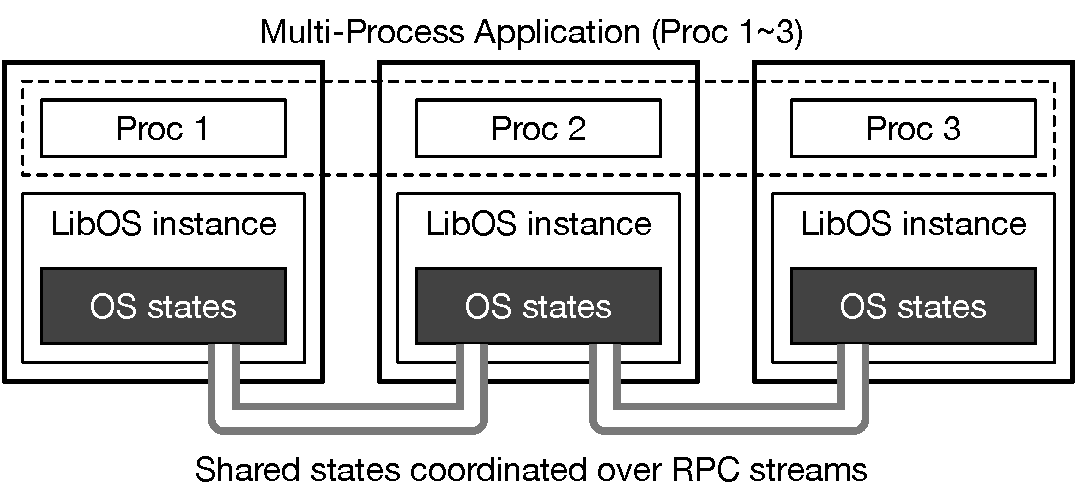
\includegraphics[width=4in]{graphene/figures/concept.pdf}
\caption[Multi-process support model of \graphene{} \libos{}]
{Multi-process support model of \graphene{} \libos{}. For each process of an application, a \libos{} instance will serve system calls and keep local OS states. States of multi-process abstractions are shared by coordinating over host-provided RPC streams, creating an illusion of running in single OS for the application.}
%\vspace{-.1in}
\label{fig:graphene:concept}
\end{figure}

{\bf \graphene{}} is a Linux-compatible library OS
to run legacy, unmodified Linux applications.
In \graphene{}, multiple \libos{} instances collaboratively implement
POSIX abstractions,
yet appear to the application
as a single, shared OS.
\graphene{} instances coordinate state using remote procedure calls (RPCs) over
host-provided byte streams (similar to pipes).
In a distributed POSIX implementation, placement of shared state and messaging complexity
are first-order performance concerns.
%We chose to shift implementation complexity into the library OS
%in order to uphold simple enforcement of security isolation in the host.
By coordinating shared states across \libos{} instances,
\graphene{} is able to create an illusion 
of running in a single OS
for multiple processes in an application (as figure~\ref{fig:graphene:concept}).
%Previous library OS designs ensured security isolation of independent applications,
%comparable to a VM, by keeping a relatively narrow host ABI.
%We selected the \graphene{}
%design because it strikes a unique balance between
%and robust, flexible security enforcement.
The \graphene{} design ensures security isolation of
mutually distrusting, multi-process
applications on the same host system.
Essential to this goal is
minimally expanding the host ABI to support multi-processing,
as well as leveraging RPCs as a natural point to mediate inter-\picoproc{} communication.
RPC coordination among \graphene{} instances can be dynamically disconnected, facilitating novel sandboxing
techniques.  For instance, we develop an Apache web server extension that, upon logging in a given user,
places the worker process's \libos{} in a sandbox with access to only that user's data.
We expect more nuanced degrees of trust are possible in future work.

\begin{comment}
The contributions of this paper are:
\begin{compactitem}
\item \graphene{}, a Linux library OS, which supports
  real-world, multi-process applications including a shell, web server,
  and compiler, which can be  efficiently checkpointed and migrated.
% \fixmetsai{We need to enable mulit-process checkpointing and migration}
% \daniela{the reviewers will be looking for that in the experiments section: "among hosts''}.
\item A framework for implementing multi-process APIs across cooperating library OS instances.
%\daniela{I would change to: "A thorough security analysis of \graphene{} isolation design'' You mention that you trust the reference momitor, so there is no security to
%be evaluated unless you guarantee the process is not vulnerable to exploits. We have not evaluated the security of the coordination design, only the isolation. To evaluate the security to the coordination design we have to look at possible race conditions and how they are dealt with.}
%\item Addressing additional challenges developing a robust Linux library OS, including copy-on-write fork.
\item A thorough evaluation of the overheads of \graphene{}.  Memory footprints are an order of magnitude
smaller than KVM, and several applications perform comparably to a Linux process.
\item A thorough analysis of \graphene{} security isolation.

%In the best case, the overhead of a large {\tt gcc} compilation on \graphene{} is only 3\%.

\end{compactitem}
\end{comment}

%\graphene{}'s design gives the user and system administrator a high degree of flexibility
%in isolating arbitrary groups of unmodified application processes,
%while upholding the efficiency and host compatibility benefits of recent library OSes.

%\fixmedp{After a complete draft is written, coalesce all goals and make sure they are addressed early on.  We are doing some scatter-shot motivation}


\section{Implementing Linux Personality}
\label{sec:graphene:background}

%Recent library OSes~\cite{porter11drawbridge,unikernels,baumann13bascule,osv}
%are designed for security and efficiency, but are limited to single-process applications.
%The security isolation of \liboses{} derives from 
%limited, explicit data sharing and 
%a narrow host interface.  
A \libos{} typically executes in either a paravirtual VM~\cite{unikernels,osv}
% \daniela{I would have the use of a VM as a discussion topic in the end of the paper.}, 
or an OS process, called a \emph{\picoproc{}}~\cite{porter11drawbridge,baumann13bascule},
with an interface restricted to a narrowed set of host kernel ABIs.
These host ABIs heavily restrict effects outside of the application's address space;
as a result, applications in a \picoproc{} have very little opportunity to interfere with each other,
yielding security isolation comparable to a VM.
Library OS efficiency comes from deduplicating features, such as hardware management;
in a VM these features typically appear in both the guest and host kernels.


\graphene{} executes within a \picoproc{} (Figure~\ref{fig:graphene:arch}),
which includes an \emph{unmodified} application binary and supporting libraries, 
running on a \libos{} instance.
The \libos{} is implemented over a host kernel ABI
designed to expose very generic abstractions that can be easily 
implemented on any host OS, including virtual memory, threads, synchronization, byte streams (similar to pipes),
a file system, and networking.
Although the \graphene{} prototype  host kernel is Linux, 
we adapt a host ABI from Drawbridge/Bascule,
which has been previously implemented on Windows, Hyper-V, and Barrelfish~\cite{porter11drawbridge,baumann13bascule,baumann09barrelfish}.
%The \graphene{} host ABI is
% summarized in Table~\ref{tab:abi} and discussed in more detail in \S\ref{sec:linux:pal}\fixmedp{if not cut...}.  
%which exposes only tens of simple host calls. \daniela{briefly define \picoproc{}: A \picoproc{} is unmodified application code running with a \libos{}.}


\begin{figure}[t]
\centering
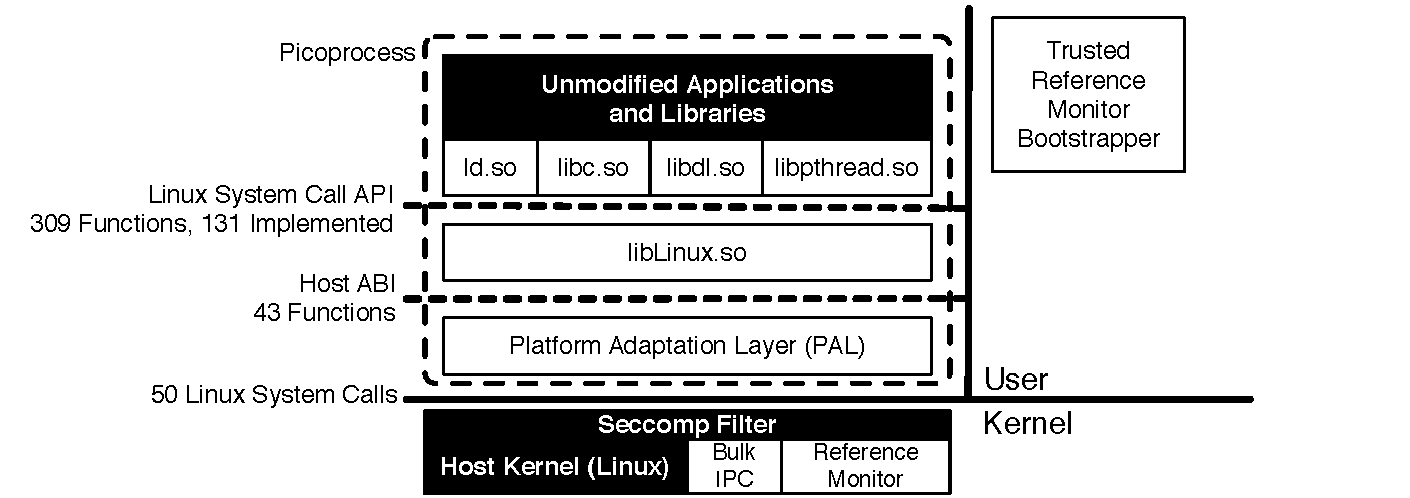
\includegraphics[width=6.5in]{graphene/figures/arch.pdf}
\caption{Building blocks of \graphene{}.  Black components are unmodified.
We modify the four lowest application libraries on Linux:
{\tt ld.so} (the ELF linker and loader),
{\tt libdl.so} (the dynamic library linker),
{\tt libc.so} (standard library C),
and {\tt libpthread.so} (standard threading library),
that issue Linux system calls as function calls directly to {\tt libLinux.so}.
Graphene implements the Linux system calls
using a variant of the Drawbridge ABI,
which is provided by the Platform Adaptation Layer (\pal{}),
implemented using calls to the kernel.
A trusted reference monitor that ensures \libos{} isolation
is implemented as a kernel module.
Another small module is added for fast bulk IPC.}
\label{fig:graphene:arch}
\end{figure}


\graphene{} exports \palcalls{} host ABIs through a 
Platform Adaptation Layer (\pal{}) (Table~\ref{tab:graphene:abi}).
The \pal{} is a binary injected into the \picoproc{} by the host, 
and translates the generic \picoproc{} ABI into host system APIs.
Most of these calls only affect the application-internal state;
any calls with external effects are mediated by a trusted \emph{reference monitor} on the host.
%The reference monitor is a trusted non-\graphene{} process running on the system.
All \graphene{} applications are launched by the reference monitor,
which installs a system call filter and interposes on permitted kernel calls to ensure isolation
(\S\ref{sec:graphene:security}).


These \pal{} ABIs should be a sufficient substrate upon which to
implement guest-specific semantics, or guest \emph{OS personality}.
As an example of this layering, consider the heap memory management abstraction.
Linux provides applications with a data segment---a 
legacy abstraction dating back to original Unix and the era 
of segmented memory management hardware.
The primary thread's stack is at one end of the data segment, and the heap is at another.  
The heap grows up (extended by {\tt sys\_brk}) 
and the stack grows down until they meet in the middle.
In contrast, the \pal{} ABI provides only three simple functions 
that allocate, protect, or unmap regions of virtual memory
with basic access permissions (read, write, and execute).
This clean division of labor encapsulates 
idiosyncratic abstractions in the library OS,
and eliminates the need for
redundant hardware management code, 
such as duplicate low-level page management and swapping heuristics.


%These interfaces are host-independent \daniela{OS or kernel-independent}, as they tend to be very generic and easily
%implemented on any host OS kernel or VMM \daniela{postpone VMM for later}.

At a high level, these library OS designs
scoop the layer just below the system call table out of the OS kernel
and refactor this code as an application library.  
The driving insight is that there is a natural, functionally-narrow division point 
one layer below the system call table
in most OS kernels.
Unlike many OS interfaces, these \pal{} ABIs generally minimize the amount of application state in the kernel, facilitating
migration: a \picoproc{} can programmatically read and modify its own OS state,
copy the state to another \picoproc{}, and the remote \picoproc{} can 
load a copy of this state into the OS---analogous to hardware registers.
A \picoproc{} may not modify another \picoproc{}'s OS state.



%% To implement the Linux OS
%% personality, we introduce 1 ABI for managing x86 segment registers and
%% 2 for handling runtime hardware exceptions.  The extensions are
%% expected to uphold host compatibility since they are also identified
%% and introduced in Bascule. In addition, 6 new ABIs, including
%% copy-on-write page exchanges, stream handle sharing, and sandbox
%% creation, are introduced to improve either efficiency or security
%% isolation of library OSes. These ABIs can always fall back to the
%% Drawbridge/Bascule ABIs if users decide to prioritize compatibility.

\begin{comment}
\begin{table}[t]
\footnotesize
\centering
\begin{tabular}{|l|c|>{\palign{l}}p{4.8in}|}
\hline
\multicolumn{3}{|c|}{\bf Adopted from Drawbridge} \\
\hline
{\bf Class} & {\bf ABIs} & {\bf Description} \\
\hline
Memory & 3 & Allocate and protect virtual memory. \\
\hline
Scheduling & 12 & Threads and synchronization. \\
\hline
Files \&  Streams & 12 & Files inside a {\tt chroot}-style; jails and byte streams among \picoprocs{}. \\
\hline
Process & 2 & Create a child \picoproc{}, and exit self. \\
\hline
Misc & 4 & Get random bits, time of day, etc. \\ % flush instruction cache, etc.\\
\hline
\multicolumn{3}{|c|}{\bf Added by \graphene{}} \\
\hline
{\bf Class} & {\bf ABIs} & {\bf Description} \\
\hline
Segments & 1 & Manage x86 segment registers (FS and GS) for TLS. \\
\hline
Exceptions & 2 & Handle hardware exceptions. \\
\hline
Streams & 4 & Share stream handles across \picoprocs{}, rename files, and set stream attributes (file permissions, socket options, etc.) \\
\hline
Bulk IPC & 3 & Exchange copy-on-write pages.\\
\hline
Sandboxes & 1 & Move into a new sandbox, with a new manifest applied. Pipes and streams that violates the new policy are closed.\\
\hline
\end{tabular}
\caption[List of host ABI functions defined in \graphene{}]
{Classes of  host ABI functions adopted from \drawbridge{}~\cite{porter11drawbridge}, 
followed by ABIs added by \graphene{}.}
\label{tab:graphene:abi}
\end{table}
\end{comment}

\fixme{Need transition to next section.}

\subsection{Multi-Process Support in Library OSes}

A key design feature of Unix is that users compose simple utilities to create
larger applications.  Thus, it is unsurprising that many popular applications for Unix or Linux
require multiple processes
--- an essential feature missing from current \libos{} designs.
%This gap is filled by the \graphene{} \libos{}, which
%extends recent \liboses{} to support multi-process applications.
The underlying design challenge is minimally expanding 
a tightly-drawn isolation boundary
without also exposing idiosyncratic kernel abstractions or
re-duplicating mechanisms \fixme{Discuss deduplicating features upfront} in both the kernel and the \libos{}.

%requires a careful balance among the competing goals of 
%efficiency, host independence, and security isolation.
%The challenge, then, is minimal expansion of

%\vspace{5pt}
%\noindent {\bf Motivating Example.~}
For example,
consider the process identifier (PID) namespace.
In current, single-process lib\-OSes, 
the {\tt getpid()} system call could simply return a fixed value to each application.
This  single-process design is isolated,
but the library OS cannot run a shell script, which requires {\tt fork}-ing and {\tt exec}-ing multiple binaries, signaling, waiting, and other
PID-based APIs.

\vspace{5pt}
\noindent{\bf Design Options.~}
Multi-process  support requires extensions to the \pal{} ABI of recent, single-process \libos{} designs.
Because multi-process abstractions, 
such as signals or System V IPC, 
tend to be idiosyncratic,
an essential problem is identifying a minimal, host-independent
substrate upon which 
to implement OS-specific abstractions.

We see two primary design options:
(1) implement processes and scheduling in 
the library OS, and (2) treat each \libos{} instance as a process, and distribute the 
shared POSIX implementation across a collection of \liboses{}.
We selected the second option, primarily because we expected this would impose fewer
requirements on the host, maximize flexibility in mapping processes 
to physical resources, and facilitate inter-process security policy enforcement. % as enforcing security policies on related processes.

Implementing processes
inside the library OS is also feasible using 
hardware MMU virtualization, similar to Dune~\cite{belay12dune},
but this reintroduces a duplicate scheduler and memory management.
Moreover, Intel and AMD have similar, but mutually incompatible MMU virtualization support,
which would complicate live migration across platforms.
None of these problems are insurmountable, and it would be interesting in future
work to compare both options.

\paragraph{Multi-Process Support in \graphene{}.}
%\daniela{Because Approach and Motivating Example are on the same level, its seems that
%you are starting a new topic under Approach, when the discussion is actually a continuation of
%Motivating Example}
In \graphene{}, multiple \libos{} instances in multiple \picoprocs{} collaborate to 
implement shared abstractions, such as 
 copy-on-write fork, signals, exit notification,
and System V IPC.
For instance, when process A signals process B on \graphene{}, A's \libos{} issues
a remote procedure call (RPC) to B's \libos{} over a host-provided byte stream (similar to a Unix pipe),
and B's \libos{} then calls the appropriate signal handler.

%%% All collaborating \libos{} instances exchange messages as needed 
%%% to provide the application with a consistent view of 
%%% shared abstractions,
%%% such as


%\graphene{} approaches multi-processing by selectively replicating state and issuing remote procedure calls (RPCs) 
%%across multiple, collaborating
%library OS instances.
%Guests may work together to provide the unmodified multi-process application with
%coordination abstractions 

%Shared abstractions on \graphene{}'s are implemented outside of the host, ensuring  host OS independence.
% by implementing these
%shared abstractions entirely
%outside of the host kernel.
%Shared abstractions are implemented outside of the host.
%From the host kernel's perspective, 
\graphene{} implements all shared abstractions in the \libos{}, and \liboses{} cooperatively manage these abstractions
over RPC streams.
Single-process applications still service system calls from local state, and \graphene{} 
includes optimizations to place state where it is most likely to be used,
minimizing RPC overheads.
The host reference monitor can easily isolate \liboses{}
by 
% \graphene{} design isolates \liboses{} by 
%requiring all coordination to use 
%explicit bytes streams \daniela{, pipe-like abstractions provided by the kernel. (suggestion: Reviewer  3)}.
%Security isolation is enforced
%by a kernel-level {\em reference monitor}, which can 
%disconnect or prevent creation of a
blocking all
RPC messages, % between \liboses{} that should be isolated,
without the need to understand the \libos{} details or semantics of these abstractions.
In our PID example, only mutually-trusting \liboses{} can signal each other.
%if the reference monitor prevents creation of RPC streams
%across mutually untrusting \picoprocs{},
%the \liboses{} cannot exchange signals.

%%% \graphene{} is designed to 
%%% The \graphene{} design leverages a number of optimizations to service application system calls 
%%% from local state whenever possible, and to minimize message passing overheads otherwise
%%%  (\S\ref{sec:namespaces:insights}).
%%% Our experience is that starting with a local system call design and then extending it to share state is relatively straightforward,
%%% and introduces little-to-no overhead when the request can be serviced locally.


The \graphene{} library OS is designed
to gracefully handle disconnection from other \liboses{}, 
facilitating dynamic application sandboxing.
RPC streams may be disconnected at any time by 
either the reference monitor or at the request of a \libos{}.
%Message streams may be severed externally, by the reference monitor, or 
%one guest may simply disconnect from others to isolate itself.
%An application may disconnect itself from the 
%Any \graphene{} application may dynamically detach from the confederation, 
%or a host-level sandbox may dynamically separate two guests by severing their communication channels.
When \graphene{} \liboses{} are disconnected, each instance will handle the subsequent
divergence 
%and the library OS will will fork these abstractions
{\em transparently} to the application.
For instance, if a child process is disconnected from the parent by the reference monitor,
each \libos{} will interpret the event as if the other process terminated---closing any open pipes,
delivering exit notifications, etc.
% \daniela{(applications run unmodified) - Reviewer 1 asked clarification on transparently}.

%% A key insight behind our design is that the common use case for these \daniela{cooperating} abstractions
%% is between a pair of processes.  Thus \graphene{} leverages a number of optimizations 
%% to reduce broadcast messages, avoid replication of needless state,
%% and service requests locally


\paragraph{Changes to \pal{} ABI.}
When implementing \graphene{},
we found that the Drawbridge ABI lacked 12 \pal{} calls
essential to running a Linux \libos{} with multi-process support, and 
\graphene{} did not require 3 \pal{} calls to support checkpoint and resume.
Of the 12 new calls, 4 are required for single-process Linux and similar ABI have also been added by \emph{Bascule}~\cite{baumann13bascule}:
rename a file, manage segmentation hardware, and 2 for exception upcalls;
5 are required for stream inheritance, attribute configuration, and sandboxing;
and 3 new calls are used to utilize Bulk IPC channel, for optimizing copy-on-write fork (\S\ref{sec:graphene:impl}).
%Our design requires only 11 additional \pal{} calls, which we believe are fundamental to executing 
%Unix-style multi-process applications.
We design these new \pal{} calls in consideration of the platform independence
among different hosts;
If a \pal{} call is added for optimizations (e.g., Bulk IPC),
it is optional if the implementation is difficult or infeasible on a host.
%in case that the new \pal{} calls are not possible to implement on a host,
%the 
%Our design deliberately provides options where these new \pal{} calls are missing, to preserve the platform importance proven by \emph{Drawbridge}~\cite{porter11drawbridge}.
For example, copy-on-write forking can still be supported
without Bulk IPC supported on the host.
Instead, the inheritance of process state for
copy-on-write forking will be completely over regular pipes.

\paragraph{Comparison with \microkernel{}s.}
The building blocks of \graphene{} are very similar to the system abstractions of a 
\microkernel{}~\cite{liedtke95sosp,klein09sel4,elphinstone13microkernels,liedtke93sosp,chen93memory,Baron:1985:MOE,Accetta:1986:MNK},
except a \microkernel{} often has a even narrower, more restricted interface
than the \pal{} ABI.
%such as the port and
%message abstractions of Mach~\cite{
Unlike a multi-server \microkernel{} system, such as GNU Hurd~\cite{hurd} or Mach-US~\cite{stevenson95mach-us},
which implements Unix abstractions across a set of daemons that are shared by all processes in the system,
\graphene{} implements system abstractions as a library in the application's address space,
and can coordinate library state among \picoprocs{} to implement shared abstractions.
\graphene{} guarantees isolation equivalent to running 
an application on a dedicated VM; this isolation could be implemented on a multi-server \microkernel{}
by running a dedicated set of service daemons for each application.

%%% \graphene{}'s differences are motivated by two considerations: efficient support of both stand-alone, 
%%% single-process applications and multi-process applications; as well as flexible security isolation. 
%%% \graphene{} contributes techniques to seamlessly and efficiently transition 
%%% between single-process and multi-process support, as well as adapting 
%%% some known techniques to a new environment.

The \graphene{} host ABI could be described as a hybrid \microkernel{},
which also exposes the file system and network of the host kernel.
Similarly, we assume that \picoprocs{} are provided by a legacy OS kernel, like Linux or Windows,
or by a Type 2 hypervisor.  We expect that a bare metal hypervisor could export a \pal{},
but would probably require services from a trusted VM, such as Xen's dom0~\cite{barham03xen}.
%or the \pal{} would implement more thread scheduling, networking, and file system code;
%or the \pal{} ABI would change to push this code into the \libos{}.
Arguably, recent \libos{} designs might be improved by rethinking the division of labor in
the network and file system stacks, but this is beyond the scope of this thesis.

\paragraph{Alternatives.}
Another approach to support multi-process applications in a \libos{} 
would be to use hardware MMU virtualization such as nested paging
used by a system like Dune~\cite{belay12dune}
in order to implement a second process abstraction, memory manager, and scheduler in the \libos{}.
This approach threatens the efficiency benefits of deduplicating these features.
A final option is exposing additional kernel interfaces, such as signals, 
by adding more system calls to a \picoproc{}.
This approach undermines host independence, as many of these coordination abstractions 
tend to be very OS-specific.
%Unix signals vs.\ Windows events, {\tt waitpid()} vs.\ blocking on a process handle, etc.
This approach also harms security isolation, as the \libos{} now has access to generally 
porous host kernel interfaces.  
%Although legacy OSes do enforce some access control rules on coordination abstractions,
%kernel developers must audit and add hooks to millions of lines of code.
%As a result,
%users have lost confidence that a traditional OS can comprehensively enforce 
%security isolation on these abstractions---a key motivation for using VMs
%for security isolation.


Systems must strike a careful balance between the competing goals of
security isolation and
multi-process coordination.
Multi-process applications require OS-managed coordination abstractions
such as signals, process exit notification, and System V IPC.
These coordination abstractions operate within shared namespaces, such as the 
process ID namespace
and the System V key space.
These coordination APIs and namespaces must be consistent among coordinating processes,
but can %introduce information leaks and 
undermine security isolation among unrelated processes on the same host.
System designs generally only meet one goal: 
traditional OSes have a rich but porous coordination interface, 
while sandboxing systems and virtual machines (VMs) 
are strictly isolated.
This thesis demonstrates that this unfortunate trade-off is not
fundamental.
%coordination or isolation.  


Traditional OS kernels typically provide  rich multi-process coordination 
APIs, but this richness also makes for a very porous attack surface
area.  For instance, on Windows, a program may inject libraries and
create threads in another program~\cite{windows-dll-inject}; 
similarly, unchecked file descriptor inheritance in Linux can lead to
security problems~\cite{close-on-exec}.  
Although legacy OSes do enforce some access control rules on these abstractions,
kernel developers must audit and add hooks to so much code
that
users have lost confidence that an OS can comprehensively enforce 
security isolation on these abstractions.

For achieving strong security isolation on applications,
%generally lost confidence that legacy OSes can robustly enforce security isolation, and 
users have turned to virtual machines (VMs).
For instance, if two customers host their websites in the same cloud service,
the customers will insist on running their web servers in separate VMs for security.
VMs take a heavy-handed approach to security isolation --- ensuring 
that every application has a dedicated OS kernel in a hardware-isolated address space.
Although virtual machines isolate
applications and provide legacy OS abstractions within a VM, 
coordinating applications must be statically placed in the same VM,
and cannot dynamically move to a separate VM.
For instance, consider a web service running
inside of a VM that wishes to isolate requests for different users in
different VMs after authentication.  The web server administrator must
statically create a VM for each user, introducing substantial
overhead; and the developer loses convenient IPC abstractions and
must rewrite large swaths of code.

\section{Isolating Mutually Untrusting Applications}
\label{sec:graphene:security}

\sysname{} ensures that mutually untrusting applications 
cannot interfere with each other, providing security isolation
comparable to running in separate VMs.
\sysname{} reduces the attack surface exposed to applications
by restricting access to the host kernel ABI 
and prevents access to unauthorized system calls, files, byte streams,
and network addresses with a \term{reference monitor}.
%The host kernel ABI exported by the \pal{} heavily 
%limits the ability of a \sysname{} application to interact with the rest of the system;
%any external interactions are further mediated by a reference monitor.
%Unlike a typical Linux system, \sysname{} applications cannot interact with shared 
%system daemons or other shared system resources.
%As a result, \sysname{} enforces security isolation similar to running applications in separate VMs---even
%applications that span multiple processes.
\sysname{} contributes a multi-process security model 
based on the abstraction of a \term{sandbox},
or a set of mutually trusting picoprocesses.
The reference monitor permits picoprocesses within the same sandbox
to communicate and exchange RPC messages, but disallows cross-sandbox communication.
The current work focuses on all-or-nothing security isolation, although we expect
this design could support
controlled communication among mutually untrusting \liboses{}
in future work.

The only kernel-level sharing abstractions the reference monitor must mediate
are files, network sockets, and RPC streams
--- all other allowed kernel ABIs
modify only local \picoproc{} state.
%Thus, the reference monitor need only mediate file access, socket and RPC stream creation.
%an unprivileged daemon
%as well as extensions to the App\-Armor LSM~\citep{apparmor},
%which checks file and socket policies in the kernel.
%, reducing context switching overhead
%and the risk of race conditions~\citep{garfinkel03traps}.
In order for the reference monitor to restrict file access, socket and RPC stream creation,
each application includes a \term{manifest file}~\citep{hunt07rethink},
which describes a {\tt chroot}-like, restricted view of the local 
file system (similar to Plan 9's unioned file system views~\citep{pike90plan9}),
%including read-only shared files,
as well as \term{iptables}-style~\citep{iptablesman} network restrictions.
%%% To facilitate sharing read-only libraries,
%%% a manifest may specify a file system view which 
%%% combines several different sub-directories of the local file system,
%%% and can prevent writing to files or directories.


%The \sysname{} reference monitor on a Linux host
%is implemented using {\tt ioctl} system call to a special device {\tt /dev/graphene}.
%A picoprocess is restricted by seccomp filter~\citep{seccomp} to use any {\tt open} or socket {\tt connect} and {\tt bind} system calls.
%It must use the \sysname{} special device to open or create streams,
%so the file paths or network addresses can be checked against the sandbox rules.
%The kernel module as the driver of the \sysname{} special device can coexist with any LSM such as \term{AppArmor} or \term{SELinux}.


\fixme{Explain with a figure.}
When a new picoprocess is launched by the reference monitor, it begins execution in 
a new sandbox.  
Child picoprocesses may either inherit their parent's sandbox, 
or can be started in a separate sandbox
--- specified by a flag to the picoprocess creation ABI.
A parent may specify a subset of its own file system view 
when creating a child, but may not request access to new regions of the 
host file system. 
%The restrictive policy enforced on the child will be written in a new manifest file generated by the parent, and the policy will be checked by the reference monitor.
The child may also issue an {\tt ioctl} call to 
dynamically detach from the parent's sandbox. The reference monitor prevents byte stream creation 
across sandboxes.
%among picoprocesses
%that are not in the same sandbox.
%and restricts external connections to remote URIs according to firewall rules in the manifest.
When a process detaches from a sandbox --- effectively splitting the sandbox ---
the reference monitor closes
any byte streams that could bridge the two sandboxes.

\paragraph{Threat Model.}
We assume  a trustworthy host OS and reference monitor,
which mediates all system calls with effects outside of a picoprocess's address space,
such as file {\tt open} or network socket {\tt bind} or {\tt connect}.
We assume that picoprocesses inside the same sandbox trust each other and that all untrusted code runs in sandboxed picoprocesses.
We assume the adversary can run arbitrary code inside of
one or more picoprocesses within one or more sandboxes.
The adversary can control all code in its
picoprocesses, including {\tt libLinux} and the \pal{}. 
%We also assume a trusted reference monitor process running on the host kernel that 
%launches \sysname{} applications and mediates all system calls with external effects,\fixmedp{define precisely}

\sysname{} ensures that %The key security property the \sysname{} design upholds is that 
the adversary cannot interfere with any victim picoprocesses
in a separate sandbox.  
The \sysname{} sandbox design ensures strict isolation: 
if the only shared kernel abstractions are byte streams and files, 
and the reference monitor ensures
there is no writable intersection between sandboxes,
the adversary cannot interfere with any victim picoprocess.


%%% The only processes allowed to run as standard kernel processes (non-\sysname{}) 
%%% are the reference monitor and
%%% system administration utilities that need more kernel interfaces than the \pal{} ABI provides.
%%% Ensuring that a collaborating picoprocess correctly implements
%%% some function (such as receiving a signal),
%%% as well as preventing exploitation of vulnerabilities in picoprocesses
%%% are beyond the scope of this work.

\sysname{} reduces the system attack surface of the host, but does not change the size of its
trusted computing base; however, reducing the effective system call table
size of a picoprocess does facilitate adoption of a smaller host kernel,
which we leave for future work.

\subsection{System Call Restriction}
\label{sec:graphene:security:syscalls}


Unmodified Linux applications run on \sysname{} by issuing 
system calls as library calls to {\tt libLinux}.
Application calls are serviced by {\tt libLinux}-internal data structures
or \pal{} calls.
The \pal{} is implemented using \nativecalls{} host system calls.
The host OS must block any 
native system call that 
does not appear in the \pal{} source code.
Any allowed system call with external effects is checked by 
the reference monitor.
 
%% dp: Meh
%%% Any picoprocess implementation 
%%% must restrict access to the host system call table,
%%% generally by blocking system calls in the host kernel~\citep{porter11drawbridge}
%%% or using {\tt ptrace}~\citep{xax}.


%The \pal{} is a host-provided library which implements \palcalls{} generic kernel ABIs,
%implemented using 
%These native system calls include {\tt ioctl} with 5 opcodes exclusively used by \sysname{} kernel extensions.

%This section describes how we adapt recent Linux sandboxing techniques 
%to \sysname{}.


%all allowed system calls with potentially external effects.

%%% For instance, an attempt to open a file will be checked by the reference monitor
%%% to see if the file is included in the sandbox definition, specified in the manifest
%%% with required permissions.
%%% Once the file handle is open, the \pal{} is then allowed to issue an {\tt mmap} or {\tt read}
%%% on the handle, as this operation can only affect the picoprocess address space
%%% or  file, which was already checked.

%Because the \pal{} is in the same address space as the application code, it is not
%trusted to enforce any security policies, and our threat model assumes that
%the \pal{} can be compromised by the adversary.
%Thus, the host kernel 
%only permits system calls that appear in the \pal{}'s source code and, through the reference monitor, further inspects calls that can have external effects.

\begin{figure}[t!]
\centering
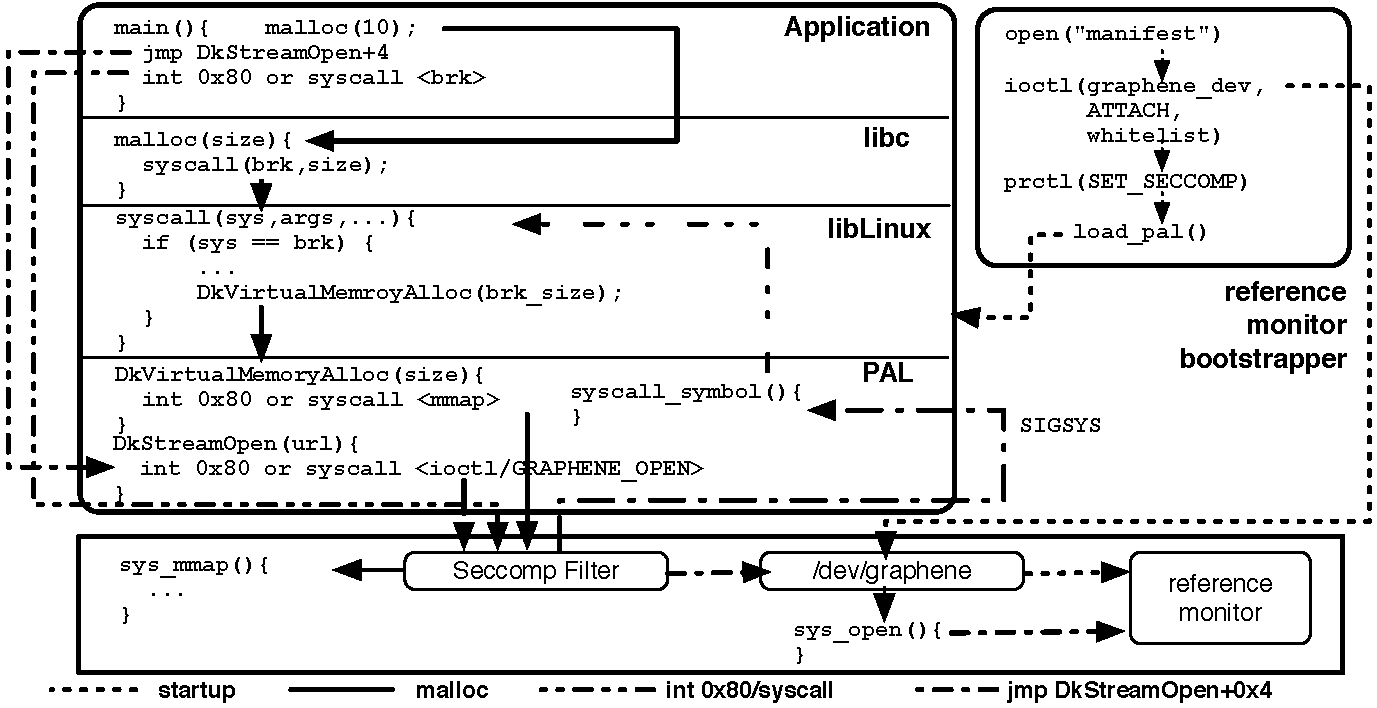
\includegraphics[width=6.5in]{graphene/figures/syscall-restriction.pdf}
\footnotesize
\caption[System call restriction approach in sysname{}]
{System call restriction approach. The reference monitor loads policies into the LSM at startup.  A \sysname{} application requests OS services in three different ways. 
In the normal case (first line of {\tt main}), {\tt malloc} is invoked causing the invocation of {\tt brk} ({\tt libLinux}) and {\tt mmap} in the \pal{}. In the second line, the application jumps to an address in \pal{}, which is permissible.
Files are accessed through {\tt ioctl} to {\tt /dev/graphene} and checked by reference monitor.
The third line invokes {\tt brk} with an {\tt int} instruction, which is redirected to the {\tt libLinux} function.}
\label{fig:graphene:syscall-restriction}
\end{figure}



\sysname{} restricts the host system call table 
using seccomp~\citep{seccomp}, introduced in Linux 2.6.12.
% a recent Linux system call filtering mechanism, called 
Seccomp allows a process to create an immutable Berkeley Packet Filter (BPF) program
that specifies allowed system calls, as well as creates {\tt ptrace} 
events on certain system calls.
The filter can also filter scalar argument values,
such as only permitting specific {\tt ioctl} opcodes.
%The BPF grammar is rich enough to filter system calls by 
%This feature is particularly salient in the case of {\tt ioctl},
%where the \pal{} uses 5 out of over 400 opcodes for our bulk IPC module and sandbox creation;
%our BPF rules will block any other {\tt ioctl} opcode.
If a system call is rejected, the \pal{} will receive a {\tt SIGSYS} signal,
and can either terminate the application or redirect the 
call to {\tt libLinux}.
Seccomp filters cannot be overridden by any picoprocess,
and are always inherited.
% by all descendant processes.
The current \sysname{} filter is 79 lines 
of straightforward BPF macros.  In our experience, adding more precise argument checks
has not significantly changed performance.

%Seccomp filters are installed using the {\tt prctl} system call;
%blocking {\tt prctl} in a seccomp filter prevents further changes to the filter.

Unfortunately, the logic to check for allowed paths network addresses cannot be implemented 
as a seccomp rule, because it involves reading user memory of unknown sizes. 
In order to avoid the overhead of trapping to the reference monitor on 
every use of {\tt open}, {\tt stat}, {\tt bind} or {\tt connect} system calls, we instead 
force picoprocess to only use {\tt ioctl} system call to \sysname{} special device ({\tt /dev/graphene}) as alternative interface these system calls. Direct access to these system calls are banned by seccomp filter.
%extend AppArmor~\citep{apparmor} 
%to enforce file system isolation in the kernel.

In order to reduce the impact of bugs in the reference monitor,
the reference monitor itself runs with a seccomp filter,
blocking unexpected system calls.

\paragraph{Static Binaries.} 
For compatibility with statically linked binaries, which 
compile in system call instructions,
we leverage seccomp to redirect these calls 
back to {\tt libLinux}.  
For system calls that could also be issued by the \pal{},
we augment our BPF rules with program counter-based filters.
In other words, an {\tt open} system call with a return PC address inside the \pal{} 
will be sent to the reference monitor for further inspection;
an {\tt open} system call with any other return PC address generates 
a {\tt SIGSYS} and is ultimately relayed back to {\tt libLinux}.
Thus, {\tt libLinux} can catch and differentiate application-issued system calls
from those that could also be issued by the \pal{}.
We hasten to note this feature is only for backward compatibility,
not security. 


\begin{comment}
We hasten to note that program counter filtering
is only provided for backwards compatibility, not security.
An attacker can compromise the \pal{}, so system policies are enforced
externally by the reference monitor.


Dynamically redirecting system calls to {\tt libLinux} is 
less efficient than dynamically linking against
the \sysname{} libc or statically compiling {\tt libLinux} into the application.
The overhead of dynamic redirection comes from 
transferring control to the kernel, then back to 
the \pal{}, and then to {\tt libLinux}.
We leave exploration of more efficient alternatives for future work,
such as redirecting the hardware system call table to {\tt libLinux}
on a host system like Dune~\citep{belay12dune},
or dynamically rewriting parts of the static binary~\citep{hunt99detours}.
\end{comment}

\paragraph{Example.}
Figure~\ref{fig:graphene:syscall-restriction} illustrates three possible situations. 
%% An unmodified Linux application is dynamically linked against the 
%% \sysname{} {\tt libc}, 
%% which then dynamically links its system calls from {\tt libLinux},
%% which in turn links in the host kernel ABI from the \pal{}.
%% The application requests OS functionality in three ways.
An unmodified application first invokes the {\tt libc} function {\tt malloc}, which issues 
a {\tt brk} system call to {\tt libLinux}, which requests memory 
from the host via a {\tt Dk\-Virtual\-Memory\-Alloc} \pal{} call,
which ultimately issues an {\tt mmap} host system call.
The {\tt mmap} host system call is allowed by seccomp because it only 
affects the picoprocess's address space.
The second line of the application jumps to the \pal{} instruction that issues
an {\tt open} system call.
From a security perspective, this is permissible,
as it is isomorphic to \pal{} functionality.
In practice, this could cause
corruption of {\tt libLinux} or application data structures,
but the only harm is to the application itself. 
Because this system call involves the file system, the reference monitor LSM first checks if the file to be opened is included in the sandbox definition (manifest) before allowing  the {\tt open} system call in the kernel.  
Finally, the application uses inline assembly to issue a {\tt brk} system call;
%in an attempt to obtain I/O port privilege; 
because this system call was not issued by the \pal{},
seccomp will redirect this call back to the \pal{},
which then calls the {\tt libLinux} implementation.

\paragraph{Process-specific Isolation.} 
Sandbox creation in \sysname{} can provide
more options than virtualization, to reflect the security policy of applications at any timing,
in the granularity of picoprocess. 
A picoprocess can voluntarily detach itself from the current sandbox, dropping its privileges,
after finishing security-sensitive operations.
If a picoprocess decides one of its children is not trustworthy, it may also start the child under a restricted manifest,
or promptly shut down RPC streams to stop sharing OS states.
The picoprocess that moves to a separate sandbox will have a restrictive view of the filesystem, and no coordination with the previous sandboxes.
In section~\ref{sec:graphene:eval}, we describe an experiment that improves security isolation of Apache web server without sacrificing functionality.

\subsection{Reference Monitor}
\label{sec:graphene:security:monitor}

The reference monitor is a trusted process that runs on the host system.
\sysname{} applications are launched by the reference monitor,
which instantiates the seccomp filter and traces all children
to check host system calls that could have external effects.
The reference monitor interposes using ptrace events, 
which can be raised for specific system calls by seccomp.
We ensure that all processes created within a sandbox are traced
by setting the {\tt PTRACE\_O\_TRACESECCOMP} option on all newly created picoprocesses
in the sandbox.

%% from bpjain:
% We have to set the option PTRACE\_O\_TRACESECCOMP on new children
% using ptrace(PTRACE\_SETOPTIONS) and we get the event as
% PTRACE\_EVENT\_SECCOMP whenever a syscall that is Traced is called.
% It happens before the grandchild starts running. We get the
% notification of creation of grandchildren by setting ptrace option
% PTRACE\_O\_TRACECLONE on the child(i.e., parent of grandchild).  I
% need to monitor every fork/clone (only clone since pal only calls
% clone). I get this event even if fork/clone is just allowed.  And
% the event that arrives on clone/fork is completely different from
% seccomp event. Thats a ptrace event too.. but we get
% PTRACE\_EVENT\_CLONE whenever a clone is done by a child on which
% PTRACE\_O\_TRACECLONE option was set.

Each application includes a \term{manifest file}, which specifies restrictions,
including network firewall rules and subsets of the host file system sandboxed
applications are permitted to access.  The reference monitor enforces these
rules by interposing on all system calls involving file paths or remote network addresses.
%\fixmedp{Revise if we can do something smarter; 2x check implementation status before submission}.

%% dp Sadface :(
\paragraph{Privilege.~} 
Although the reference monitor is trusted, it does not run 
with administrative privilege.
Linux 3.5, which we use as our host kernel, 
introduced the {\tt NO\_NEW\_PRIVS} bit, which permits
a non-privileged process to impose sandboxing restrictions on a child.
%Ubuntu back-ported this feature to Linux 3.2, which we use as our host kernel.
This flag prevents a process from acquiring root privilege, % (e.g., via executing a {\tt setuid} binary),
is inherited by all descendant processes,
and cannot be disabled.

\paragraph{Creating New Sandboxes.~} We add a \pal{} call which
permits a picoprocess to request that it be moved into a new sandbox.
This call, as well as file system path checks, are implemented
as extensions to the  AppArmor LSM~\citep{apparmor}.
%We modify \sandboxmodlines{} lines in the
%to implement this call,
The new sandbox call closes any open stream handles that cross sandbox boundaries;
mediate path lookups;
and create a new broadcast stream for multi-process
 coordination (\S\ref{sec:graphene:namespaces:blocks}).
%The reference monitor also interposes on this call so that it can 
%mediate future stream creation.

To securely apply seccomp filtering we leveraged the fact that all
\sysname{} processes have the same parent and also the new
{\tt NO\_NEW\_PRIVS} bit introduced for Linux processes starting kernel
version 3.5. This bit can be set by any process, is inherited across
{\tt fork}, {\tt clone}, and {\tt execve}, and cannot be unset by
children processes. Thus, we set the {\tt NO\_NEW\_PRIVS} bit in the initial
\sysname{} process and apply seccomp filters allowing only system calls
with corresponding functions in the \pal{}. As a result all \sysname{}
processes will inherit the filters and cannot relax or bypass it.



%which reduces the kernel
%system call API surface to user-level processes. This mechanism allows
%a process to specify a whitelist filter for system calls, which is
%implemented as a Berkeley Packet Filter (BPF) program. The invocation
%of a disallowed system call causes the application to throw a {\tt SIGSYS}
%signal, which can be caught by a registered handler provided by the
%application. In \sysname{} we registered this handler at the \pal{}.


%\sysname{} applications rely on an OS loaded as a library to request
%system services. As most of traditional applications, \sysname{}
%processes do not normally issue system calls directly: they invoke
%wrapper functions from a \sysname{}-compliant version of libc, which
%allows for portability, security (parameters are limited and checked)
%and easiness of programming. However, while standard libc functions
%directly invoke the kernel system call themselves, our modified
%version of libc wrappers invoke functions from another library which
%represents the OS, libLinux (Figure \ref{fig:graphene:syscall-restriction}). A
%\sysname{} application can access all necessary system functionality
%through libLinux, which invokes corresponding system call functions at
%the \pal{}, also loaded as a library with a
%\sysname{} process. The \pal{} is the layer responsible for directly
%invoking system calls at the kernel. As discussed in \S\ref{sec:graphene:impl} the \pal{} provides \sysname{} applications with a
%subset of the kernel system call interface.\sysname{} applications rely
%on an OS loaded as a library to request system services.
%
%Even though we expect most of \sysname{} applications to leverage libc
%wrappers, we need to address applications that need to invoke system
%calls directly. Applications might need to bypass a library such as
%libc because some needed wrappers are not provided (there are no
%wrappers in libc for module and NUMA related system calls), or the
%wrapper does not meet the programmer’s needs. \sysname{} applications
%that need to perform direct invocation of system calls run unmodified
%as long as the system calls invoked are provided by the libos{l{}. We
%do not consider this a security violation; even though the application
%would be risking not functioning according to the libosaradigm for
%bypassing the \pal{}, all potential damage would be confined in the
%misbehaving application itself.  However, we do not allow the direct
%invocation of a system call that does not have a corresponding
%function in the libosnd \pal{}. In Figure \ref{fig:graphene:syscall-restriction}
%we illustrate these three situations. We have a \sysname{} application
%loaded with three libraries: a \sysname{}-compliant libc, libLinux
%representing the library OS with functions for a selected number of
%system calls, and the \pal{} which actually invokes host kernel system
%calls. The illustrated application requests three different types of
%OS functionality. It first invokes a function from libc, then it
%directly invokes a system call whose functionality is provided by the
%\pal{}, and third it attempts to directly invoke a system call not
%present in the \pal{}, which is not allowed by \sysname{}.

%We enforce system call restriction by leveraging seccomp Linux system
%call filtering mechanism~\citep{seccomp}, which reduces the kernel
%system call API surface to user-level processes. This mechanism allows
%a process to specify a whitelist filter for system calls, which is
%implemented as a Berkeley Packet Filter (BPF) program. The invocation
%of a disallowed system call causes the application to throw a {\tt SIGSYS}
%signal, which can be caught by a registered handler provided by the
%application. In \sysname{} we registered this handler at the \pal{}.
%
%To securely apply seccomp filtering we leveraged the fact that all
%\sysname{} processes have the same parent and also the new
%{\tt NO\_NEW\_PRIVS} bit introduced for Linux processes starting kernel
%version 3.5. This bit can be set by any process, is inherited across
%{\tt fork}, {\tt clone}, and {\tt execve}, and cannot be unset by
%children processes. Thus, we set the {\tt NO\_NEW\_PRIVS} bit in the initial
%\sysname{} process and apply seccomp filters allowing only system calls
%with corresponding functions in the \pal{}. As a result all \sysname{}
%processes will inherit the filters and cannot relax or bypass it.


%\begin{figure}
%\begin{centering}
%\includegraphics[width=2.0in\textwidth]{figures/syscall_restriction.png}
%\footnotesize
%\caption{System call restriction approach. \sysname{} application requesting OS services. The {\tt printf} function is handled by a wrapper function at our modified version of libc., which invoked a corresponding syscall function at libLinux, the library OS.This function invokes a system call function at the \pal{}, which actually invokes kernel system calls. The application also directly invokes two system calls and the last invocation is prohibited.
%\label{fig:syscall_restriction}
%\end{centering}
%\end{figure}

%\end{comment}

\section{Coordinating Guest OS States}
\label{sec:graphene:namespaces}

%\fixmedp{RF: what are the few, powerful mechanisms?  Expect that there are many cases 
%with shared state; re-read this to see if it is clear how to generalize the approach}

%Recent library OS designs focus on single-process applications,
%which move a substantial portion of the OS APIs and state used by the application into the \libos{}.

%A key contribution of the \graphene{} 
%design is robust and flexible support for multi-process applications.
An application executes on \graphene{} 
with the abstraction that all of its processes are running on a single OS.
\graphene{} \libos{}es service system calls
from local \libos{} state whenever possible,
and state is coordinated across \picoprocs{} via RPC when necessary.
Within a sandbox, \graphene{} \picoprocs{} 
coordinate shared state used to implement multi-process
abstractions, such as process identifiers, thread groups, and 
System V IPC including message queues and semaphores, shared file system and file descriptor states (Table~\ref{tab:graphene:multiproc}).
Similar to previous designs~\cite{porter11drawbridge,baumann13bascule}, 
\graphene{} uses the host file system; 
the \libos{} implements file handles and translates between POSIX and the host ABI.
Identifying the best division of labor for a \libos{} file system is 
left for future work.

\begin{comment}
\begin{table}
\footnotesize
\centering
\begin{tabular}{|p{0.9in}|p{1.5in}|p{3.6in}|}
\hline
{\bf Ab\-strac\-tion} & {\bf Shared State} & {\bf Strategy} \\
\hline
Fork & 
\raggedright
PID namespace & Batch allocations of PIDs, children generally created using local state at parent.  \\
\hline
Signaling & PID to \picoproc{} map & Local signals call handler; remote signal delivery by RPC.  Cache mapping of PID to \picoproc{} ID. \\
\hline
\raggedright
Exit notification & 
\raggedright
Remote process status  & Exiting processes issue an RPC, or one synthesized if child becomes unavailable.  The {\tt wait} system call blocks until notification received by IPC helper. \\
\hline
{\tt /proc/[pid]} & Process metadata & Read over RPC.  \\
\hline
Message Queues & 
\raggedright
Key mapping, queue contents & Mappings managed by a leader, contents stored in various \picoprocs{}.  When possible, send messages asynchronously, and migrate queues to the consumer.\\
\hline
Semaphores & 
\raggedright
Key mapping, count. & Mappings managed by leader, migrate ownership to \picoproc{} most frequently acquiring the semaphore. \\
\hline
\raggedright
File System & 
\raggedright
File truncate sizes, FIFO files, domain sockets, symbolic links, file locks & No coordination, create special files in the host to represent symbolic links and file locks. \\
\hline
\raggedright
Shared File Descriptors & 
\raggedright
Seek pointers & Mappings managed by parent, migrate ownership to \picoproc{} most frequently accessing the file descriptors. \\
\hline
\end{tabular}
\caption[Multi-process abstractions implemented in sysname{}]
{Multi-process abstractions implemented in \graphene{}, coordinated state, and implementation strategies.}
\label{tab:graphene:multiproc}
\end{table}
\end{comment}

%% Outline

% Basic idea of what we are doing
% Building blocks
% Implemented abstractions and examples (table)
%% Why not shared FDs?
% Optimizations/insights
% Why different from microkernels?


\begin{comment}
The general problem underlying each multi-process API is 
{\bf namespace management}.  Coordinating \picoprocs{} need a consistent mapping
of names, such as a thread ID or System V message queue ID, 
to the \picoproc{} implementing that particular item.  
Picoprocesses then implement abstractions such as signals
by issuing a remote procedure call (RPC) to the appropriate \picoproc{}.
Because many multi-processing abstractions in Linux can also be used by single-process applications,
a key design goal is to seamlessly transition between single-process uses, serviced 
entirely from local \libos{} state, and multi-process cases, which
leverage remote procedure calls (RPCs) to coordinate accesses to shared abstractions.

As an example of balancing security isolation and coordination APIs,
consider functionality that use the process ID namespace,
such as  Unix signaling or exit notification (e.g., {\tt waitpid()}).
In \graphene{}, the process ID namespace, 
as well as signaling and related system calls,
are implemented inside the library OS.
A process can signal itself by having the \libos{} directly call the handler function.
When \picoprocs{} are in the same sandbox, they coordinate
to implement a consistent, shared process ID namespace,
as well as to send and receive signals amongst themselves.
Cross-process signals are implemented as RPCs
over kernel-managed streams.
When \picoprocs{} are in separate sandboxes,
they do not share a PID namespace, and cannot send signals to each other.
The reference monitor ensures that IPC abstractions, such as signaling,
cannot escape a sandbox by preventing the creation of kernel-level streams
across sandboxes.
\end{comment}


%Figure~\ref{fig:sandbox} illustrates several sandboxes with \picoprocs{}
%collaborating to implement a process ID namespace.  
%Because this namespace is a guest-level abstraction,
%different sandboxes can have overlapping process IDs, and
%cannot signal each other.
%If the connection between the two \picoprocs{} on the right of the figure
%is severed by subdividing the sandbox,
%the processes will become inaccessible to each other
%and each newly isolated library OS will treat the event as a process termination.
%\fixmedp{See if we can get a better figure}

%dp:  Seems redundant, probably imported from S2
\begin{comment}
Within a sandbox, each library OS tracks the PIDs of other \picoprocs{}.
As children are created, each library OS updates its own replica of the 
process tree, with annotations for which host-level connection corresponds
to the remote process.  
If a \picoproc{} signals itself, the signal system call simply calls the 
appropriate signal handling function in the application. 
If a \picoproc{} signals another \picoproc{},
the signal essentially becomes an asynchronous remote procedure call
from the sending library OS to the receiving library OS.
Note that this is all transparent to the unmodified application.
Section~\ref{sec:graphene:namespaces} describes these library OS-internal
coordination mechanisms in more detail.
The current \graphene{} prototype supports 
a range of coordination abstractions, including signaling, 
exit notification, System V message queues, thread identifiers and groups, sessions,
and the process tree.
We believe this sample is sufficiently representative that
remaining tail of Linux IPC abstractions could be easily added.

The reference monitor ensures security isolation
simply by preventing \picoprocs{} in different sandboxes from 
sharing host-level streams.
We adopted this approach to maximize dynamic sandboxing flexibility,
rather than, say, attempt to multiplex one single library OS instance across multiple processes.
\end{comment}

\begin{comment}
A driving design insight is that the common case
for coordination is among pairs of processes.
Examples include a parent waiting on a child to exit, 
one process signaling another, or a single producer and single consumer
sharing a message queue.
Thus, \graphene{} optimizes for the common case of pairwise coordination,
reducing the overhead of replicating data (\S\ref{sec:namespaces:insights}).
\end{comment}

The rest of this section describes our coordination framework, 
beginning with the coordination building blocks,
and then explains the implementation of several multi-process abstractions.
We conclude with lessons learned from optimizing  multi-process performance.

Although a straightforward implementation worked, tuning the performance was the most challenging
aspect of this design;  we conclude with a summary of the lessons learned from optimizing the system.
We conclude with lessons learned from tuning the performance of the system.
then presenting the design and driving insights,
followed by representative examples, 
and concluding with a discussion of failure recovery.

\subsection{Coordination Building Blocks}
\label{sec:graphene:namespaces:blocks}

The general problem underlying each of these coordination APIs is 
{\bf namespace management}.  In other words, coordinating \picoprocs{} need 
a consistent mapping of names, such as a thread ID or System V message queue ID, 
to the \picoproc{} implementing that particular item.  
Because many multi-process abstractions in Linux can also be used by single-process applications,
a key design goal is to seamlessly transition between single-process uses, serviced 
entirely from local \libos{} state, and multi-process cases, which
leverage remote procedure calls (RPCs) to coordinate accesses to shared abstractions.

%Picoprocesses then implement abstractions such as signals
%by issuing a remote procedure call (RPC) to the appropriate \picoproc{}.

\graphene{} creates an  {\bf IPC helper} thread within each \picoproc{},
which exchanges coordination messages with the IPC helper threads of \picoprocs{} 
within the sandbox. %, using these broadcast and point-to-point streams.
The IPC helper
services RPCs from other \picoprocs{} and is
hidden from the application. 
GNU Hurd has a similar helper thread to implement signaling among a process's parent and
immediate children~\cite{hurd};
\graphene{} generalizes this idea to share a broader range of abstractions among any \picoprocs{}
within a sandbox.
%The IPC helpers are necessary 
%in each \picoproc{} to serve remote messages and receive responses atomically.
To avoid deadlock among application threads and the IPC helper thread, 
an application thread may not both hold locks required by the helper thread to service an RPC request
and block
on an RPC response from another \picoproc{}.
All RPC requests are handled from local state and do not issue recursive RPCs.% \fixmedp{Check this}

Within a sandbox, all IPC helper threads exchange messages using a
combination of a {\bf broadcast stream} for global coordination,
and {\bf point-to-point} streams for pairwise interactions, 
minimizing overhead for unrelated operations.
The broadcast stream is created for the \picoproc{} as part of initialization.
Unlike other byte-granularity streams, the broadcast stream sends data at the granularity of messages,
to simplify the handling of concurrent writes to the stream.
Point-to-point streams are simply byte streams between two \picoprocs{};
two processes may establish a point-to-point stream by passing handles through 
an intermediate stream or over the broadcast stream.
The handle-passing ABI is discussed further in Section~\ref{sec:graphene:impl}.
%The broadcast stream is primarily used for failure 
%recovery (\S\ref{sec:namespaces:failurerecovery}); 
%Mmost operations use point-to-point streams to minimize overheads.
If a \picoproc{} leaves a sandbox to create a new one,
its broadcast stream is replaced
with a new one, connected only to the \picoproc{} and any children created in the
new sandbox.

Because message exchange over the broadcast stream does not scale well,
we reduce the use of the broadcast stream to the minimum.
Broadcast stream is merely used for {\bf \picoproc{} identifier allocation}
and {\bf leader recovery}.

One \picoproc{} in each sandbox serves as the {\bf leader}.
The leader is responsible for subdividing each namespace among other \picoprocs{} 
in the sandbox.
For example, the leader might allocate 50 process IDs to a \picoproc{}
that wishes to create children.  The {\bf owner} of the allocation can then allocate process IDs
to children from its local allocation without further involving the leader.
For a given identifier, the owner is the serialization point for all updates,
ensuring serializability and consistency for that resource.
%%% the leader's IPC helper has the added responsibility of coordinating 
%%% global state (name allocations).
%%% Our design minimizes the role of the leader, instead distributing responsibility 
%%% to specific \picoprocs{} when practical.  
%%% If the leader crashes, 
%%% a new leader can be elected. The detail of leadership recovery is discussed in
%%% Section~\ref{sec:namespaces:leader}. 
%More detailed discussion of the \graphene{}-internal
%RPC protocol is omitted for space;
%but it 
%consists of 30 message types which 
%encode both state replication and RPC 
%messages.

\subsection{Examples and Discussion}

%This subsection describes \libos{} coordination by example.
%\vspace{5pt}
\noindent{\bf Signals.~} Inside a {\tt libLinux} instance, signals are implemented using a combination of 
{\tt sigaction} data structures %adapted from Linux
to track signal masks and pending signals;
\pal{}-provided hardware exception upcalls (e.g., for {\tt SIGSEGV});
and  RPCs for cross-\picoproc{} signals (e.g., for  {\tt SIGUSR1}).
If a process signals itself, {\tt libLinux} simply uses internal data structures
to call the appropriate signal handler directly.
%this section describes how this local model is extended with RPCs for remote PIDs.
%For cross-process signals, we use the namespace coordination mechanism.
\graphene{} implements all three of Linux's signaling namespaces:
process, process group, and thread IDs.

\begin{figure}
\centering
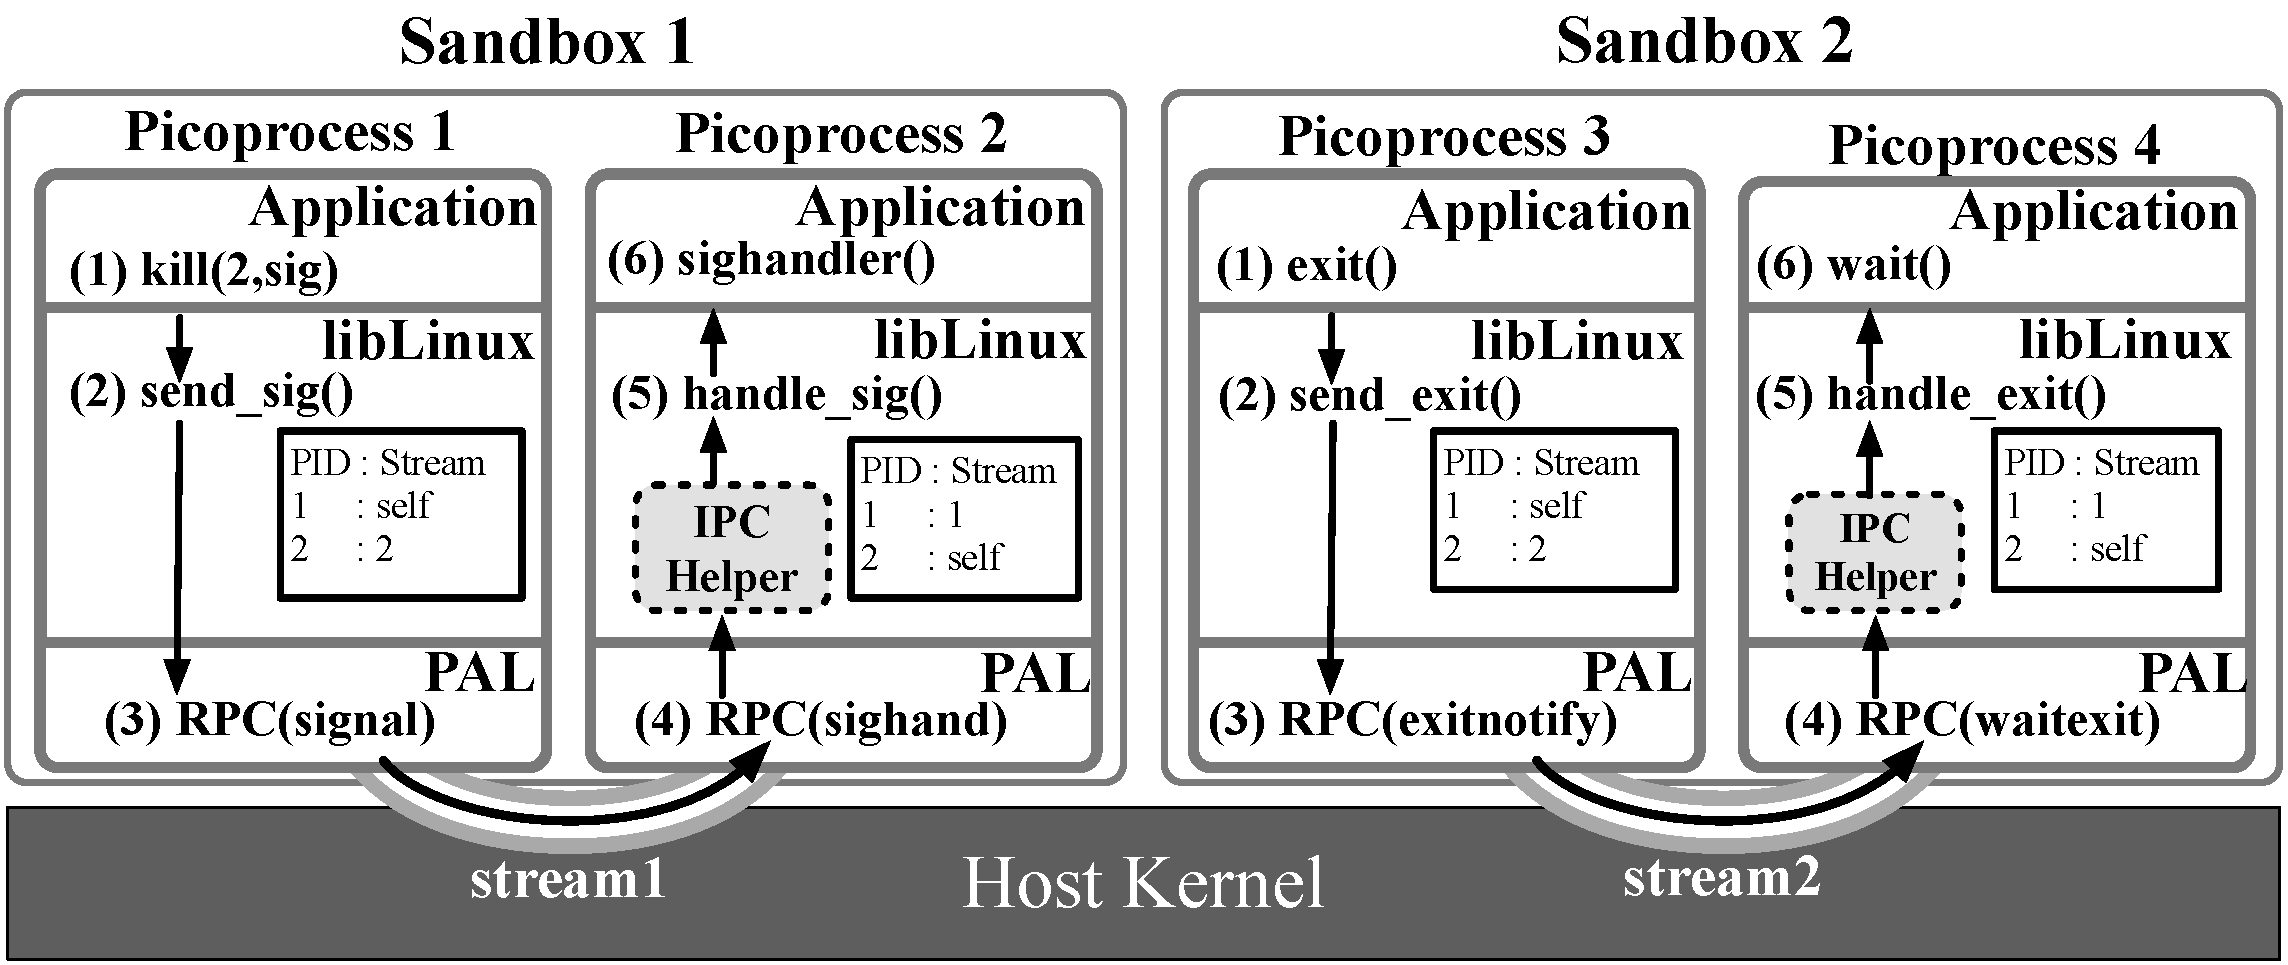
\includegraphics[width=\linewidth]{graphene/figures/coordination.pdf}
\caption{Two pairs of \graphene{} \picoprocs{} in different sandboxes 
coordinate signaling and process ID management.
The location of each PID is tracked in {\tt libLinux}; Picoprocess 1 signals
\picoproc{} 2 by sending a signal RPC over stream 1,
and the signal is ultimately delivered using a 
library implementation of the {\tt sigaction} interface. Picoprocess 4 
waits on an {\tt exitnotify} RPC from  \picoproc{} 3 over stream 2. }
\label{fig:graphene:coordination}
\end{figure}

Figure~\ref{fig:graphene:coordination} illustrates two sandboxes with \picoprocs{}
collaborating to implement a process ID (PID) namespace.  
Because PIDs and signals are a \libos{} abstraction,
\picoprocs{} in 
each sandbox can have overlapping PIDs, and
cannot signal each other.
Picoprocesses in different sandboxes cannot 
exchange RPC messages or otherwise communicate.
%If the connection between \picoprocs{} 1 and 2 is severed by subdividing the sandbox,
%the processes will become inaccessible to each other
%and each newly isolated library OS will treat the event as a process termination.


If \picoproc{} 1 (PID 1) sends a {\tt SIGUSR1} to \picoproc{} 2 (PID 2), illustrated in Figure~\ref{fig:graphene:coordination},
the {\tt kill} call to {\tt libLinux} will check its cached mapping of PIDs to 
point-to-point streams.
If {\tt libLinux} cannot find a mapping, it may begin by sending a query to the leader
to find the owner of PID 2,
and then establish a coordination stream to \picoproc{} 2.
%The leader may also pass a point-to-point coordination stream handle.
Once this stream is established, \picoproc{} 1 can send a  
signal RPC to \picoproc{} 2 (PID 2).
When \picoproc{} 2 receives this RPC, 
{\tt libLinux} will then query its local {\tt sigaction} 
structure and mark {\tt SIGUSR1} as pending.
The next time \picoproc{} 2 makes a {\tt libLinux} call,
the {\tt SIGUSR1} handler will be called upon return. Also in Figure~\ref{fig:graphene:coordination}, \picoproc{} 4 (PID 2) waits on 
\picoproc{} 3 termination (in the same sandbox with PID 1). When \picoproc{} 3 terminates, it invokes the library implementation of exit, which issues
an {\tt exitnotify} RPC to \picoproc{} 4.
%In this example, \picoprocs{} in different sandboxes have the same PID number, but this does not cause conflict as they are isolated and can only communicate with processes in the same sandbox.

%%% Using a helper thread alongside each process to asynchro-
%%% nously handle signaling
%%% is common in many \microkernel{}-based OSes such as GNU Hurd~\cite{hurd}.
%%% GNU Hurd also maintains local mappings of PIDs and RPC ports for inter-process messaging.
%%% However, PID namespace in GNU Hurd is only tracked between the parents/children, so signaling cannot be transferred between arbitrary processes.
%%% \graphene{} handles PID namespace with global consistency inside a sandbox,
%%% but requires no intensive RPCs to any centralized service.   

The \graphene{} {\tt libLinux} signal semantics closely match Linux behavior, which
delivers signals upon return from a system call or an interrupt or trap handler (\pal{} upcall).
%Each process and thread have {\tt sigaction} structures adapted from the Linux source 
%that implement the
%POSIX specification, including handler functions, as well as masking signals and
%reentrant behavior.
The {\tt libc} signal handling code is unmodified on \graphene{}.
%We extend the \pal{} with ABIs for explicit upcalls on certain hardware exceptions, such
%as divide-by-zero or segmentation faults.
%Signals from other processes, such as {\tt SIGUSR1}, are generally delivered upon 
%return from a call into {\tt libLinux}; 
If an application has a signal pending for too long,
e.g., the application is in a CPU-intensive loop, {\tt libLinux} can use a \pal{} function to interrupt 
the thread. 


% Daniela Oliveira commented. old caption for coordination
%\caption{\graphene{} namespace coordination example.  
 % Two applications and {\tt libLinux} instances
 % coordinate signaling and process ID management.
 % The location of each PID is tracked in {\tt libLinux};
 % a signal message is sent over a host stream
 % using the {\tt action} message, 
 % and the signal is ultimately delivered using a 
 % library implementation of the {\tt sigaction} interface.
%}


\begin{comment}
\graphene{} internally indexes point-to-point handles using PIDs.
In order to facilitate reallocation of PIDs without global coordination, 
\graphene{}-internal PIDs also include a {\em generation number},
allowing \picoprocs{} to lazily detect reuse similar to generation numbers 
for inodes in NFS~\cite{sandberg85nfs}.
\end{comment}

\paragraph{System V IPC.} System V IPC
maps an application-specified key onto a unique identifier.
All System V IPC abstractions, including message queues and semaphores,
are then referenced by this identifier (ID).
Similar to PIDs, 
%In order to service IPC requests, including identifier creation, from local state,
the leader divides the ID space among the \picoprocs{}, so that any \picoproc{}
can allocate an ID from local state. %a pre-allocated range.
The leader also dynamically allocates keys to \picoprocs{}.
%%% Global coordination is required to ensure that the same key maps to the same queue ID;
%%% the leader caches this information, but the owner of the queue ID or the semaphore ID 
%%% makes the definitive decision about whether a ID mapping is still valid.
%%% A key which does not have a valid mapping can be assigned to an ID by any \picoproc{}.

\paragraph{Message Queues.} In \graphene{}, the owner of a queue ID is responsible for 
storing the messages written to the queue; all message sends and receives must 
go through the owning \picoproc{}.  
In our initial implementation, any sends to or receives from a remote queue were several
orders of magnitude slower than an access to a local queue.
This led to two essential optimizations.  
First, sending to a remote
message queue was made asynchronous.  In the common case, the sender can simply assume 
the send succeeded, as the existence and location of the queue have already been determined.
The only risk of failure arises when another process deletes the queue.
When a queue is deleted, the owner sends a deletion notification to all other \picoprocs{}
that previously accessed the queue.
If a pending message was sent concurrently with the deletion notification 
(i.e., there is an application-level race condition), 
the message is treated as if it were sent after the deletion and thus dropped.
The second optimization migrates queue ownership from the producer to the consumer,
which must read queue contents synchronously.

%\fixmedp{bill: it is referenced in the Semaphores section, but here there isn't any talk about migrating msg queues to the most active \picoproc{}. also, the section starts with ``two essential optimizations. First \ldots'', but there isn't a second. is queue ownership migration the second?}

Because non-concurrent processes can share a message queue,
our implementation also uses a common file naming scheme to serialize message queues to disk.
If a \picoproc{} which owns a message queue exits, 
any pending messages are serialized to a file,
and the receiving process may request ownership of the queue from the leader.
%In order to prevent happens-before violations in case of failure, 
%message queues may be checkpointed more aggressively.


%\paragraph{Failure Recovery.}
%\label{sec:namespaces:failurerecovery}
%The \graphene{} coordination protocols are designed such that the leader does not store any unrecoverable information---the leader
%only caches the current name allocations.
%Because we assume that \picoprocs{} within a sandbox trust each other, 
%a new leader can simply broadcast a request to 
%recreate the current name allocations.  
%If the leader crashes, a simple leader election protocol is sufficient, e.g., picking the smallest live PID.

%\daniela{I wonder if the remainder of this section should be part of implementation details(section 5)}

\paragraph{Semaphores.} IPC semaphores 
follow a similar pattern to message queues, where ownership of a given semaphore is migrated
to the \picoproc{} that most frequently acquires the semaphore.
%If the owner of a semaphore exits, \graphene{} transfers ownership to the leader.  rather than serialize the semaphore to disk.
Most of the overhead in the Apache benchmark (\S\ref{sec:graphene:eval:perf}) is attributable to semaphore overheads.
%and, in ongoing work, we will likely optimize this by 
%either expanding the host ABI to share synchronization primitives within a sandbox,
%using shared memory to reduce semaphore latency.

\paragraph{Shared File Descriptors.} 
Open handle descriptors in the \graphene{} host ABI do not include a seek pointer; 
Unix-style seek behavior is implemented in the library OS.
The default Linux behavior is that children copy the open handles and file seek cursors,
but subsequent cursor movements are not shared between parent and child.
Shared file descriptor table can be requested by passing the {\tt CLONE\_FILES} flag to the {\tt clone} system call.
Any new file descriptor opened in a shared table will be visible by every process cloned in this way, as well as subsequent cursor update.
%None of our target applications have required a shared seek cursor, and it is not currently implemented,
%but would be a straightforward extension to current RPC mechanisms.
%We expect that the current RPC mechanisms could easily be extended to synchronize a seek pointer among \picoprocs{}.
If multiple \picoprocs{} are sharing file descriptor table,
the oldest one will coordinate the mapping of each file descriptor to the child \picoproc{} who owns the seek pointer.
Every update to the seek pointer will require coordination
if the \picoproc{} isn't owning it,
and similar optimization using migration can be applied here. 

\paragraph{File System States.} 
In some cases file system states need to be shared across \picoprocs{},
but the host ABI cannot export the result of Linux-specific behaviors.
For example, Linux allows user to perform specialized operations on file system
such as opening a FIFO, binding a domain socket, creating a symbolic link,
or atomically locking a file.
Coordinating these states can be cause significant slowdown on regular file system operations, so we simply export the state in regular files on the host,
 and atomically update them by renaming.

\paragraph{Shared Memory.} The \graphene{} host ABI 
does not currently permit shared memory among \picoprocs{}.
We expect that a host ABI and existing support for coordinating System V IDs would be sufficient to implement this,
with the caveat that the host must be able to handle sandbox disconnection gracefully, perhaps converting the pages to copy-on-write.
Thus far we have avoided the use of shared memory in the {\tt libLinux} implementation, both to maximize flexibility in placement of \picoprocs{}, potentially on different physical machines,
and as a rough mechanism to keep all coordination requests explicit.
%As discussed with semaphores, shared memory may also be useful to reduce latency for RPCs among picoproceses when 
%all \picoprocs{} are on the same host.


%in \graphene{} are implemented by a simple producer-consumer model.
%%% Without blocking, the latency of an inter-process semaphore operation equals to a round-trip of RPC messages.
%%% We observed that IPC semaphores can benefit from the same optimization
%%% used by message queues,
%%% based on asynchronous sending.
%%% However, when non-concurrent processes share a semaphore, it does not worth serializing the semaphore state to disk.
%%% When the owner of a semaphore exits,
%%% the semaphore state will be migrated to the leader,
%%% if it has a non-zero counter.
%%% IPC semaphores are intensively used in Apache web servers with a multi-process model. 

 
\begin{comment}
\paragraph{Limitations.} At the time of submission,
\graphene{} does not recover from all cases where a leader \picoproc{} crashes.
Our current prototype requires the IPC helper thread in the leader to remain 
in the sandbox and respond to messages even if its process {\tt main} routine has completed,
and the evaluation data reflects this state.
\end{comment}

\paragraph{Failure and Disconnection Tolerance.}  
\graphene{} is designed to tolerate disconnection of collaborating \libos{} instances,
either because of crashes or blocked RPCs.  In general, \graphene{} makes 
these disconnections isomorphic to a reasonable application behavior,
although there may be some edge cases that cannot be made completely transparent to the application.

In the absence of crashes, placing shared state in a given \picoproc{} introduces the risk that an errant 
application will corrupt shared \libos{} state.  The \microkernel{} approach of 
moving all shared state into a separate server process is more resilient to this problem.
Anecdotally, \graphene{}'s performance optimization of migrating ownership to the process that 
most heavily uses a given shared abstraction also improves the likelihood that only the corrupted
process will be affected.  
Making \graphene{} resilient to arbitrary memory corruption of any \picoproc{} is left for future work.


\paragraph{Leader Recovery.}
\graphene{} provides a leadership recovery mechanism when a leader failure is detected.
A non-leader \picoproc{} can detect the failure of a leader by either observing the shutdown of RPC streams or timing out on waiting for responses. 
Once the \picoproc{} detects leader failure, it sends out a message on the broadcast stream to volunteer for leadership.
After a few rounds of competition, the winning \picoproc{} becomes the new leader and recover the namespace state by recollecting from every other \picoproc{} in the sandbox.

%After a \picoproc{} being elected as the leader,
%the leader state,
%including all the allocated IDs and the RPC stream addresses,
%must be recovered. 
%Recollecting the leader state from all the \picoprocs{} is possible
%but can be inefficient,
%given the new leader may not have knowledge about every \picoproc{}.
%To simplify the implementation,
%we make the leaders of a namespace periodically serialize their states to disk for later recovery.

%When a \picoproc{} is sandboxed, it will detect the failure of leader because all of its RPC streams are closed by the reference monitor.
%Once it starts the leadership recovery, it will automatically win because no other \picoproc{} is sharing the broadcast stream. The procedure can be skipped by informing the sandboxed \picoproc{} before detaching.

\subsection{Lessons Learned}
\label{sec:graphene:namespaces:insights}

The current coordination design is the product of several iterations, which began 
with a fairly simple RPC-based implementation. %, and was then refined based on profiling.
This subsection summarizes the design principles that have emerged from this process.
%We present high-level facets of the design along with the insight
%behind the decision.  The next subsections synthesize these aspects 
%with specific examples of signaling and message queues.

\paragraph{Service requests from local state whenever possible.}
Sending RPC messages over Linux pipes is expensive;
this is unsurprising, given the long history of 
work on reducing IPC overhead in microkernels~\cite{liedtke93sosp,chen93memory}.  
We expect that \graphene{} performance could be improved on a 
\microkernel{} with
a more optimized IPC substrate, such as L4~\cite{liedtke95sosp,klein09sel4,elphinstone13microkernels};
we take a complementary approach of avoiding IPC if possible.
%but this is beyond the scope of our work, and we want \graphene{} to perform well on any 
%host OS.

An example of this principle is migrating message queues to the ``consumer'' when a 
clear producer/consumer pattern is detected, or migrating semaphores to the most frequent requester.
In these situations, synchronous RPC requests can be replaced with local function calls, improving
performance substantially.  For instance, migrating ownership of message queues 
reduced overhead for message receive by a factor of $10\times$.

\paragraph{Lazy discovery and caching improve performance.}  
No library OS keeps a complete replica of all distributed state,
avoiding substantial overheads to pass messages replicating irrelevant state.
Instead, \graphene{} incurs the overhead of discovering the owner of a name
on the first use, and amortizes this cost over subsequent uses.
Part of this overhead is potentially establishing a point-to-point stream,
which can then be cached for subsequent use.
For instance, the first time a process sends a signal, the helper thread 
must figure out whether the process id exists, to which \picoproc{} it maps,
and establish a point-to-point stream to the \picoproc{}.
If they exchange a second signal, the mapping is cached and reused, amortizing this 
setup cost.  For instance, the first signal a process sends to a new processes
takes \~{}2ms, but subsequent signals take only \~{}55 \us{}.

\paragraph{Batched allocation of names minimizes leader workload.}
In order to keep the leader off of the critical path of operations like {\tt fork}, 
the leader typically allocates larger blocks of names, such as process IDs or System V queue IDs.
In the case of {\tt fork}, if a \picoproc{} creates a child, it will request a batch of 
PIDs from the leader (50 by default).  Subsequent child PID allocations will be made from the same 
batch without consulting the leader.
Collaborating processes also cache the owner of a range of PIDs, avoiding 
leader queries for adjacent queries.

%% dp: Sad to see this go, but it is sort of subsumed by the other discussion
\paragraph{The coordination within a sandbox is often pairwise.}
\graphene{} optimizes the common case of pairwise coordination,
by authorizing one side of the coordination to dictate the abstraction state,
but also allows
more than two processes to share an abstraction.
Based on this insight, 
we observe that {\em not all shared state need be replicated by all \picoprocs{}}.
Instead, we adopt a design where one \picoproc{} is authoritative for a given name (e.g., a process ID or a System V queue ID).
For instance, all possible thread IDs are divided among the collaborating \picoprocs{},
and the authoritative \picoproc{} either responds to RPC requests for this thread ID (e.g., a signal)
or indicates that the thread does not exist.
This trade does make commands like {\tt ps} slower, 
but optimizes more common patterns, such as waiting for a child to exit.

\paragraph{Make RPCs asynchronous whenever possible.} 
For operations that must write to state in another \picoproc{}, 
the \graphene{} design strives to cache enough information in the sender 
to evaluate whether the operation will succeed, thereby obviating the 
need to block on the response.  This principle is applied to lower the overheads
of sending messages to a remote queue.


%this is a mapping to a thread within a specific \picoproc{}; for a message queue key,
%the mapping might be empty if the queue does not exist, or it may point to the \picoproc{} storing the pending messages.
%% The general problem underlying each of these coordination APIs is 
%% {\bf namespace management}.  In other words, coordinating \picoprocs{} need a consistent mapping
%% of names, such as a thread ID or System V message queue ID, to the authoritative \picoproc{} for that abstraction, if one exists.


\paragraph{Summary.}
The current \graphene{} design minimizes the use of RPC,
avoiding heavy communication overheads in the common case.
This design also allows for substantial flexibility to dynamically moving processes out of
a sandbox.  Finally, applications do not need to select different 
library OSes {\em a priori} based on whether they are multi-process or single-process---\graphene{}
automatically uses optimal single-process code until otherwise required.

\section{Implementation Details in \graphene{}}
\label{sec:graphene:impl}

\paragraph{Linux \pal{}.}
The majority of \pal{} calls are simple wrappers for similar Linux system calls, 
adding less than 100 LoC on average for translation between \pal{} and Linux abstractions.
The largest \pal{} calls are for exception handling, synchronization, and picoprocess
creation, which require multiple system calls and range from 500--800 LoC each.
Creating a new picoprocesses internally requires a {\tt vfork} and {\tt exec} of a clean 
application instance, and would be more efficiently implemented in the kernel.
Finally, the other major \pal{} components are an ELF loader (2 kLoC), headers (800 LoC),
and internal support code (2.3 kLoC).

\paragraph{Alternative \pal{} Ports.}
We prove the platform independence of \graphene{}
by porting \pal{} to \emph{FreeBSD}, \emph{OSX} and \emph{Windows}.
With the alternative host \pal{}, unmodified Linux binaries,
along with {\tt glibc} and {libLinux},
can be transparently run on the host.
For FreeBSD,
only 1.2 kLoC of the host \pal{} code need to be rewritten,
which are significantly less than FreeBSD Linux compatibility module (10.8 kLoC).
\pal{} components including ELF loader and internal support code can be shared by any \pal{} ports.

%\fix{We leave host \pal{} ports to non-unix OSes like Windows as future work,
%but previous works~\cite{porter11drawbridge,baumann13bascule} have already shown it feasible.}

\begin{table}[t!b!]
\footnotesize
\centering
\begin{tabular}{|l|rr|}
\hline
{\bf Component} & {\bf Lines} & ({\bf \% Changed})\\
\hline
GNU Library C ({\tt libc}, {\tt ld}, {\tt libdl}, {\tt libpthread}) & \libclines{} & $0.07\%$ \\
\hline
Linux Library OS ({\tt libLinux}) & 31,112 & \\
Linux host \pal{} & 11,644 & \\
Extra code for Linux \sgx{} host \pal{} & 9.354 & \\
% updated by Chia-Che on Oct. 10, 2013
\hline
%Storage Server & \fixmedp{XX} & \\
Reference monitor bootstrapper & \reflines{} & \\
Linux kernel reference monitor module ({\tt /dev/graphene}) & \sandboxmodlines{} & \\
Linux kernel IPC module ({\tt /dev/gipc}) & \gipclines{} & \\
\hline
\end{tabular}
\caption[Lines of code written or changed in \graphene{}]
{Lines of code written or changed to produce \graphene{}.  Applications and other libraries are unchanged.}
\label{tab:graphene:loc}
\end{table}


%% * most calls are a wrapper, \fixmedp{XX} LoC on average.
%% * Exception handling, sync, and process creation were harder (500-800 LoC each).  Process creation requires a clean instance (vfork+exec), would be simpler to implement in kernel.
%% * Other major components: ELF loader (2kLoC), headers(800 LoC), internal support code (2300 LoC)


%\fixmedp{Chia-Che, update LoC table}

\paragraph{Implementing Linux Personality.} 
%\fixmedp{Revisit the logical flow of these paragraphs}
The \graphene{} {\tt libLinux.so} implements a subset 
of the Linux system call API (currently \graphenesyscalls{} calls)
using only the \pal{} ABI to interact with the host.
We note that Linux exports a very long tail of infrequently used calls.
%applications.
A rough analysis of this tail indicates roughly 100 additional calls that can be implemented
with the existing \pal{} ABI and coordination framework, less than 10 administrative calls that will not make sense to expose to 
an application, such as loading a kernel module or rebooting the system, and roughly 54 that will require 
\pal{} extensions to meaningfully implement, such as controlling scheduling,
NUMA placement, I/O privilege, and shared memory.
In the last category of system calls, the degree to which actual host details should be exported versus emulated is debatable.

%We believe represent the most commonly used system calls.
%When an application requests a call or argument that {\tt libLinux.so} does not implement,
%the picoprocess exits with a distinct error message. 
Each time we have tested \graphene{} with a new application, the number of extra system calls
required has dropped---most recently we only added 4 calls
(namely, epoll\_create, epoll\_wait, semget and semop)
to support the Apache web server.
Thus, we believe \graphene{} implements a representative sample of Linux calls.

%such as {\tt sched\_setparam}, which manipulates scheduler-specific
%parameters or 
%{\tt uselib}, which has been abandoned 
%in {\tt glibc} version 2 in favor of a user-space dynamic linker.
%We do not plan to implement administrative interfaces, such as {\tt reboot}.
%The growth in the set of supported system calls has been driven by 
%the requirements of new applications we use to exercise \graphene{}, and has been 
%slowing considerably over time.

%directly to guests, and thus will not implement them in {\tt libLinux.so}.

% dp: :(
\begin{comment}
Most {\tt libLinux.so} code reimplements
Linux kernel functionality.  We found it expedient to 
read the Linux source in order to understand its behavior and then reimplement 
that behavior on the \pal{} ABI in most cases.
In some cases, such as the file caching code,
%directory entry (dentry) cache, 
we refactored code directly from the Linux kernel.
%% In these cases, we simplified data structures to only include data
%% we needed for a single application, and to hook in with other 
%% {\tt libLinux} subsystems.
%% An interesting direction for future work would identify techniques
%% to automatically import larger swaths of Linux kernel code, facilitating
%% adoption of new features and bugfixes.
\end{comment}

In order to use {\tt libLinux.so}, we modified \libclines{} lines of {\tt glibc} to replace 
system instructions with function calls into {\tt lib\-Linux.so},
and to cooperatively manage thread-local storage with {\tt libLinux.so} (Table~\ref{tab:graphene:loc}).

%All totaled, we only needed to modify \libclines{} lines of glibc source code to redirect all 
%system calls to {\tt libLinux} 

%\section{User-level {\tt fork} and other Linux library OS challenges}
%%% \vspace{5pt}
%%% \label{sec:fork}
%%% \noindent {\bf Copy-On-Write Fork.~}
%%% Creating a clean guest eases reasoning about security isolation, as all shared abstractions
%%% must be implemented using explicit data streams  between guests.
%%% This section describes how we implement these Unix abstractions in the guest
%%% %achieve a sensible division of labor between guest and host, and 
%%% without baking Unix personality into the host ABI.


\begin{comment}
\vspace{5pt}
\noindent{\bf Guest self-migration.~}  One of the key features of the host ABI
is that guest state can be programmatically read and recreated.
As a result, guests can checkpoint, migrate, and resume themselves in a new picoprocess,
potentially on a new host.  
Most of the library OS and application state are checkpointed simply 
by copying the contents of virtual memory into a file.
Checkpointing requires manually serializing a few key data structures
in {\tt libLinux} that are needed to resume the library OS from a checkpoint,
% interface directly with the PAL, 
including the thread states, handle table, and memory mappings.  

Resuming from a checkpoint involves restoring these key data
structures (handles, thread register contexts, memory mappings), and re-loading memory
contents from the checkpoint.  Most additional data structures
in {\tt libLinux}, and all application data structures,
are reloaded at the virtual address as before the checkpoint and work without modification.
\end{comment}

\begin{comment}
When a new guest begins execution, an input argument to {\tt libLinux} indicates
whether control should be transferred to the Linux loader ({\tt ld.so}) to start a new application instance, 
or whether a checkpoint should be loaded instead.
\end{comment}
%After the checkpoint is loaded, all threads resume execution on their stacks.

\paragraph{Implementing fork by (Ab)using Checkpoints.} 
Copy-on-write fork presented a particular challenge.
%when implemented using only a VM-like picoprocess abstraction.
As with a virtual machine, each new picoprocess 
is created in a ``clean'' state; fork is implemented in the \libos{}.
%yet applications require common Unix abstractions such as file handle inheritance and copy-on-write fork.

Graphene implements file Unix-style {\tt fork}
by leveraging portions of the checkpoint and migration code,
which can programmatically save and restore OS state (e.g., file handles, and memory mappings).
Rather than writing the checkpoint to a file, 
we developed an efficient bulk IPC mechanism to 
permit copy-on-write sharing of memory pages among processes.
Bulk IPC is a performance optimization over sending each byte of the parent address
space over a stream, although {\tt libLinux} can also implement {\tt fork}
over a stream.
Bulk IPC adds 3 calls to the host ABI,
and the host reference monitor only permits bulk IPC among
picoprocesses within a sandbox.

%% Conceptually, {\tt fork} could be implemented by checkpointing the parent,
%% modifying the primary thread's checkpoint 
%% so that the child returns 0 from the fork call 
%% (indicating it is the child),
%% and then immediately resuming the checkpoint in another picoprocess.

%% In practice, we optimize {\tt fork} performance by avoiding 
%% the use of an intermediate checkpoint file, instead transferring the checkpoint
%% directly to the child over a host-level bulk IPC
%%  mechanism (\S\ref{sec:linux:pal}).
%The Graphene bulk IPC abstraction adds 3 PAL calls 
%that allow guests to efficiently transfer large regions of memory to each other\fixmedp{after reordering, add a forward or back ref}.

Using our bulk IPC mechanism,
the sender (parent) can request that the host kernel copy
a series of pages, which need not be virtually contiguous,
into the receiver's address space.
The receiver (child) specifies where these pages should be mapped.
In both sender and receiver, the pages are marked copy-on-write.  
This bulk IPC mechanism sends pages out-of-band on a byte stream and guests also use the stream to send control messages 
indicating 
how many pages are being sent and how they should be interpreted.

Our IPC module is \gipclines{} lines of code (Table~\ref{tab:graphene:loc}), 
runs on multiple versions of Linux (2.6 and 3 series kernels), and
does not require
Linux kernel changes or recompilation.


\begin{comment}
A critical challenge in developing a Linux library OS was implementing 
handle inheritance in the guest.  In some cases, 
handles are easy to reproduce: an open file can simply be reopened in the child,
and the cursor offset adjusted (note that file handle offsets are a library abstraction
implemented over a memory mapped file).
Pipes, however, are not easily recreated without host support.
\end{comment}
%One option was to create explicitly named host-level byte streams,
%similar to System V or Windows named pipes.
%This strategy is simple to add to the Drawbridge host ABI and easy to program in {\tt libLinux},
%but complicates security isolation, as guests must be prevented from 
%opening a host-level pipe outside of their sandbox.

%A second option, which we pursue, is to only create anonymous bytes streams,
\paragraph{Inheriting File Handles.}
Graphene adds two PAL ABI functions that transfer 
stream handles out-of-band over reviously 
established byte streams within a sandbox.  Handle passing facilitates inheritance
and general-purpose RPC.
This mechanism is similar to Unix Domain Sockets,
which are commonly used by sandboxing systems. % such as plash~\citep{plash}.
This strategy allows a guest to seamlessly and explicitly 
share an open handle with another guest in the same sandbox, but prevents
a guest from sharing a handle with a guest outside of the sandbox.

\begin{comment}
\vspace{5pt}
\noindent{\bf Discussion.~}
A Graphene picoprocess can copy part or all its address space into a child
picoprocess relatively efficiently.
Although this mechanism is less efficient than an in-kernel {\tt fork},
we wanted to maintain the generality benefits of recent \liboses{},
and only added the minimal building blocks to the host ABI.
%we felt this design would bake Unix personality into the host kernel ABI,
%and  reintroduce security problems caused by accidental inheritance~\citep{close-on-exec}.
The transfer of data is explicit to the host, can be mediated by a reference monitor,
the sender, or the receiver.
For instance, recent Unix systems introduced a close-on-exec flag for file handles~\citep{close-on-exec}, 
which prevents inheritance of handles to sensitive files.  This can be implemented
either in a parent, by excluding the file handle from a checkpoint, 
or in the child, by closing this handle on an {\tt exec} call.
Our current implementation implements close-on-exec in the child for complete compatibility,
but a more security-sensitive application could easily implement ``close-on-fork'' semantics 
in the parent.
This clean division of labor retains full functionality
and facilitates extensibility.


\end{comment}


\begin{comment}
\vspace{5pt}
\noindent{\bf ABI Extensions.~}
\graphene{} extends the Drawbridge ABI with 9 additional \pal{} calls.
As discussed above, one creates a new sandbox, and 
5 additional calls were added for IPC.
We also add 3 calls to manage x86 segmentation registers
and exceptions (Bascule~\cite{baumann13bascule} adds
similar extensions).
\end{comment}

\paragraph{Synchronization.} Perhaps surprisingly, implementing Linux
synchronization appears substantially easier than Windows synchronization, 
as {\tt libLinux} did not require all of the various
synchronization ABIs provided by Drawbridge.
We believe the reason for this is that Linux has consolidated 
all user-level synchronization primitives to use futexes~\cite{franke02futex},
which are essentially kernel-level wait queues.
%In Windows parlance, this is simply an Event associated with a virtual address.
%Thus, our effort implementing synchronization was relatively straightforward.

%\papersection{\Thehostabi{}}
\label{sec:overview:host}

\issuedone{1.1.b}{Describe \thehostabi{} specification}
The development of \graphene{} starts with defining a simple host ABI (application binary interface) called \thehostabi{},
containing only OS abstractions essential to target applications.
%and is easily ported to different platforms.
%and minimal specifications for the host OSes and hardware.
%The host ABI is a new boundary between OSes (or hypervisors) and applications.
\Thehostabi{} separates
the implementation of an existing system API (application programming interfaces), which determines the compatibility against applications,
from hardware abstraction features, such as file systems, network stacks, and device drivers. 
\graphene{} moves the system API components
to a \libos{} in the userspace and reimplements the functionality using \thehostabi{}.
To port \graphene{} to a new host OS or hardware,
OS developers only have to implement \thehostabi{} on the target host system API,
%to new host OSes and hardware,
instead of paying a tremendous cost to translate the whole system API specification. Figure~\ref{fig:overview:porting} illustrates the porting process of \graphene{}.



%The host ABI separates the low-level, hardware management features, from the idiosyncrasy of system interface. 
%\graphene{} moves the upper layer of OS components,
%including the system calls and namespaces, into an library OS,
%leaving \thehostabi{} 
%as a narrowed interface to the host OSes and hardware.
%The host ABI intends to minimize the development effort on each host OS or hardware
%to mitigate the interface distinctions,
%to simply porting the OS abstractions defined in \thehostabi{}.


\begin{figure}[t!]
\centering
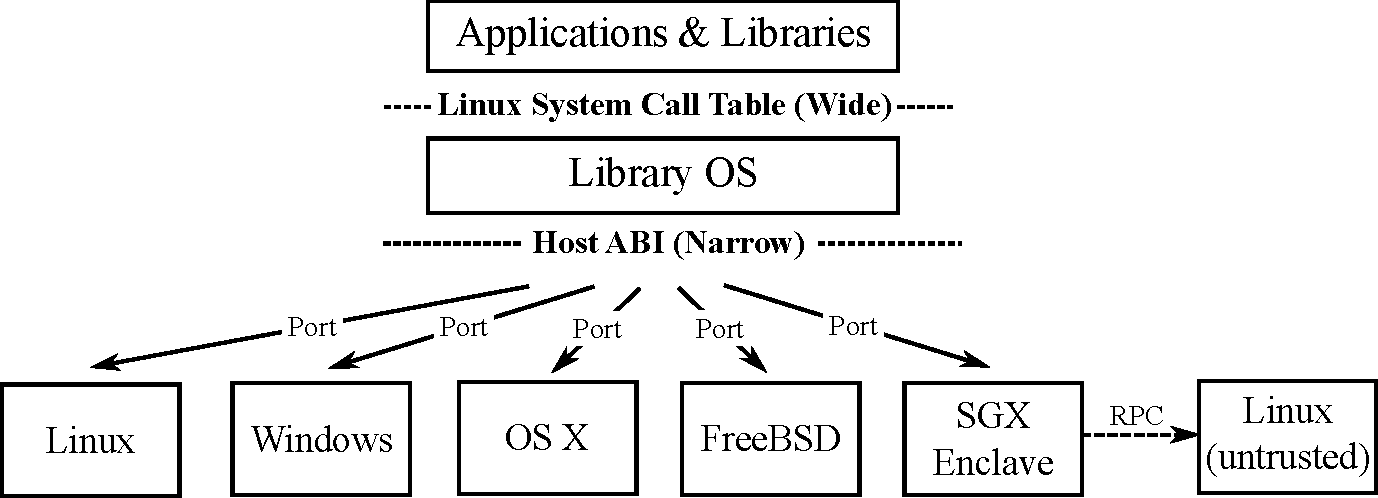
\includegraphics[width=30em]{porting.pdf}
\caption{Porting model of \graphene{}.}
%\vspace{-.1in}
\label{fig:overview:porting}
\end{figure}



\papersubsection{Platform Adaption Layers (PALs)}
\label{sec:overview:host:pal}


For each host OS or hardware, \graphene{} uses
a thin library called a {\bf platform translation layer (PAL)}
to translate among host interfaces.
%is loaded below the library OS, to translate each functions in \thehostabi{} to native system interfaces.
The main purpose of a PAL is to mitigate the semantic gap
between \thehostabi{} and
native host system APIs.
%The effort of PAL development is per host OS, whereas the library OS implementation is reusable on every hosts. %The simplicity of \thehostabi{} can be also estimated by the effort of implementing a PAL for each host.
By implementing a PAL on a new host OS or hardware,
users can reuse
the same \libos{} to run the same collection of unmodified Linux applications.
%To keep the porting effort low,
%the development of a PAL must be straightforward
%for average OS developers.
%to achieve with limited efforts.
%Based on the principle of porting simplicity, PAL development must be straightforward
%for average developers.







%The host ABI is defined for the simplicity of porting, as well as the sufficiency for implementing a library OS compatible to Linux.
%First of all, the number of host functions included in \thehostabi{}
%is much smaller than the number of system calls in a commodity OS such as Linux. 
\graphene{} currently contains PAL implementations for several popular OSes,
including Linux, \win{}, \osx{}, and FreeBSD.
%and \sgx{} with an untrusted Linux kernel.
Most of these OSes provide a POSIX-like system API similar to \thehostabi{}.
Due to the similarity, translating most of \thehostabi{} to one of the system APIs
are straightforward for average OS developers.
\Thehostabi{} is also much smaller than the actual POSIX API, making it extremely portable.



A part of \thehostabi{} may be challenging to port
on an OS,
due to unexpected system assumptions made by the OS.
For instance, \win{} does not support
fine-grained memory deallocation for de-privileged applications.
To implement system calls like \syscall{munmap} and \syscall{mprotect},
\graphene{} needs host ABIs to
deallocate or protect virtual memory pages at page granularity.
%A workaround is to change memory mappings at the physical page level,
%but will require running the \win{} PAL with root permissions.
%This type of porting challenges
%tends to be results of design decisions or assumptions made by OS developers.
%A \libos{} can potentially design
%different emulation strategies
%to compensate missing host abstractions.
A few host abstractions such as a bulk IPC feature are
optional to the host ABI;
if a host OS does not support these abstractions,
the \libos{} must fall back to alternatives. 

%In our experience, the development of a PAL is around ten thousand lines of code.

%For each port, the amount of code written for implementing \thehostabi{} is at the order of magnitude of thousands of lines of code, which is much more manageable than implementing a flat translation layer for system interfaces.


\begin{comment}
Based on the experience in \graphene{},
it is hard to ensure the portability of \thehostabi{} on every potential hosts.
%even a host ABI specialized for simplicity cannot guarantee to be portable on every hosts.
A host may simply lacks the functionality
for implementing a \hostapi{}.
The assumption is, maintaining the compatibility of \thehostabi{} poses a much less challenge than maintaining the whole system API.
Besides, the library OS may flexibly switch among emulation strategies
to compensate the absence of certain host abstraction.
As an example,
bulk IPC is optional in \thehostabi{} since its first definition,
due to the expectation
that implementing the feature may not be feasible on some hosts.
If bulk IPC is not available,
the library OS can fall back to RPC-based IPC, with a reasonable amount of performance penalty.
In the worst case, if there is no emulation strategies
to compensate for the absence of a \hostapi{},
user can predict the affected applications and avoid running these applications
on specific hosts. 
%at least users can predict whether an application will be affected and thus cannot run on certain hosts.
\end{comment}


%For a host OS that does not support ELF binaries, the PAL must follow the binary format which the host OS accepts, such as the Portable Executable (PE) format on \win{}.
%The PAL is the only layer in the user space which cannot be reused
%across different hosts. Besides the PAL, all of the other binaries in the user space are fully reusable, including the library OS, the supporting libraries, and the application executable.



%The host abstractions map to several common system calls in a commodity OS.
%For example, \funcname{StreamRead} and \funcname{StreamWrite} can directly map to the POSIX functions \funcname{pread} and \funcname{pwrite}, which are available in most OSes including Linux, BSD, \osx{}, and \win{}.
%More than half of the functions in \thehostabi{} can be counted toward this category.
%The rest of the host abstractions are either specific to Linux
%(e.g., TLS support),
%or belong to the POSIX functions that are not shared with commodity OSes
%(e.g., \funcname{mmap} on \win{}).
%The PAL emulates these host abstractions, using existing system interfaces available on the host OS, unless the software emulation is fundamentally impossible (e.g., restricted by the system interfaces), or too expensive (e.g., high overhead from copying data).



\papersubsection{Definitions and design principles}
 

\graphene{} defines \palcallnum{} calls in \thehostabi{} (also called \hostapis{}),
with a set of host abstractions
sufficient for \libos{} development.
%The host ABI defines the interaction between the library OS and a specific host.
%The \graphene{} library OS can be deployed on any ``host'' where \thehostabi{} has been ported.
This thesis defines
a {\bf host} of \thehostabi{}
to be an OS or hypervisor
which contains enough OS functionality for running a standalone application or virtual machine.
Most of the host targets in \graphene{}
are monolithic OSes,
including Linux, \win{}, \osx{}, and FreeBSD.
%which has defined a massive system API for programmability.
A monolithic OS 
usually contains a massive amount of system APIs,
which is sufficient for
implementing \thehostabi{}.


A special example of a host
is an \sgx{} (Software Guard Extensions) enclaves~\cite{intelsgx},
which
restricts OS functionality for security reasons.
The restrictions on \sgx{}
are results of a strong threat model
which distrusts any OS features except ones that are virtualized by the CPUs or migrated into enclaves.
The only way to obtain any missing OS features such as storage or networking
is to request through RPC (remote procedure call).
Requesting untrusted OS services through RPC also introduces new security threats that application developers tend not to anticipate~\cite{checkoway13iago,osdi16scone}.
Due to all the compatibility and security challenges discussed above,
this thesis uses \sgx{} as a representative example of a host
with unusual assumptions (e.g., threat models) and restrictions
compared to a monolithic OS.

%An innovative hardware abstraction like \sgx{} (software guard extensions)
%imposes unique assumptions and restrictions
%on a commodity OS,
%%creates a special host on top of Linux or \win{},
%%with unique interfaces and specifications regarding the host OSes.
%and thus creates a special host above the OS.

%If an OS has mutated or tweaked the interface for a hardware platform,
%such as an \sgx{} enclave 
%running on an untrusted Linux kernel,
%the combination of the OS (Linux) and the hardware platform (\sgx{}) is considered a specialized host.
%Especially, the \sgx{} port of \thehostabi{} faces several unique challenges,
%which will be discussed in Chapter~\ref{chap:sgx}.


\begin{comment}
%\fixme{each sentense should be a paragraph; starting the 2nd sentence}
\fixmedp{start with a strong opening stating the rationale}
The host ABI of \graphene{}
define functions needed from a host, in order to implement the library OS for reusing applications.
%to reuse an application and all its supporting libraries, including the \graphene{} library OS.
Each host of \graphene{} contains an OS and a hardware platform, either of which causes compatibility issues for running unmodified applications.
OS developers can port the library OS to a new host,
by simply reimplementing the narrowed host ABIs using abstractions available on the host.
%a new host platform.
%For each host which requires the compatibility for unmodified Linux applications, one only has to implement the narrowed host ABIs,
%instead of reimplementing the bloated, ``legacy'' system interfaces
%needed by the applications.
By implementing \thehostabi{}, OS developers skip the painful process of rebuilding the whole system interfaces of a commercial OS such as Linux.
The host ABIs strictly decouples the porting effort on the hosts from the compatibility feature for applications.
%The host ABIs decouple the OS development in the host and the implementation of compatibility for the existing Linux application.
What \thehostabi{} exposes is a simplified extended machine,
similar to a para-virtualization interface, capable of running the library OS as a lightweight virtual machine. % with compatibility against Linux applications.
%on which another layer of virtualization (i.e., the library OS) can be built to reproduce the compatibility for Linux.
\end{comment}


\begin{comment}
Two design principles drive the definition of \thehostabi{}s:
{\em simplicity} (i.e., easy to port on any hosts)
and {\em sufficiency} (i.e., containing enough OS functions for implementing a library OS).
The process of deciding \thehostabi{}s is comparable to
finding a ``pinch point'' within a OS implementation,
which can conveniently mediate a significant portion of OS execution paths for managing hardware abstractions.
%The two principles drive the development of \thehostabi{}s,
%The whole development of the \graphene{} library
%must be disciplined
%on extending \thehostabi{}s only when it is strongly required.
%of restraining extensions to \thehostabi{}s unless absolutely necessary.
The two principles
determine the soundness of the \graphene{} approach to improving compatibility
for any hosts.
\end{comment}


%%The host ABI is defined with partitioning in mind.
%\Thehostabi{} 
%determines a boundary which partitions several upper-level OS components, %, such as system calls and namespaces,
%into a library OS,
%%, as a dynamically-linked library which can be deployed
%%to various hosts.
%%The rationale behind the partitioning is based on the fact that not every OS component is equally important to compatibility, for applications which need to be ported across hosts.
%%When an OS is extended for a new hardware,
%%these OS components usually remain unchanged, or are predominantly reused.
%%Partitioning
%%into a library OS further guards these 
%in order to isolate the host idiosyncrasy. % on specific hardware. %any potential changes for adopting new hardware.
%%Similar isolation
%%exists in traditional OSes, but without partitioning:
%The strategy
%is also used in OSes:
%An example is the Linux virtual file system (VFS), an internal interface
%which encapsulates operations of file system drivers.
%%On the other hand,
%%drivers (e.g., drivers for file systems, block devices, or network cards)
%%and architecture-specific instructions
%%stay encapsulated in the host OS.
%%in the Linux kernels are usually encapsulated under a virtualized, in-kernel interface (e.g., the Linux virtual file system),
%%to simplify the development of the rest of the kernel.
%Similar to VFS,
%\thehostabi{} is intended
%to be a more ubiquitous interface,
%which encapsulates
%any host-specific behavior and semantic
%inside the host OS.
%%for encapsulating both OS and hardware idiosyncrasy on a wide range on hosts.
%%declares a ubiquitous system interface, to encapsulate both OS and hardware abstractions
%%for the library OS.




\Thehostabi{} shares several characteristics with a virtual hardware interface
exported by a hypervisor.
A generic, backward-compatible
virtual hardware interface
%a set of generic, virtual hardware,
%which the VM can control with the same drivers.
allows an unmodified OS kernel to run inside a virtual machine as on the bare metal.
%by exporting interfaces close to commodity hardware.
%To avoid additional porting effort, the virtual hardware are close to the typical commodity hardware.
%For instance, a virtual hardware interface
%usually includes a virtual NIC (network interface controller),
%such as the virtualized E1000 interfaces
%available in VMware workstation or QEMU.
%As a result, \thehostabi{} contains the
%typical OS features and interfaces, similar to the API of early UNIX systems.
The key difference between
a virtual hardware interface
and \thehostabi{}
is that \thehostabi{} does not target reusing a whole, unmodified OS kernel as a guest.
Instead, 
\thehostabi{} contains higher-level abstractions such as files and network sockets
to ensure portability on most host OSes.
The concept
of defining \thehostabi{}
with a customized guest OS (i.e., a \libos{}) running atop \thehostabi{} is similar to para-virtualization.
%\thehostabi{} expects the \libos{}
%to be rewritten and
%customized for \thehostabi{},
%similar to a 
%para-virtualizated VM.
%Compared to an actual para-virtualized VM,
A para-virtualized VM defines hypercalls as interfaces between a guest OS and a hypervisor.
Furthermore, \thehostabi{} avoids duplication of OS components
such as scheduler, page fault handler, file systems, and network stacks
between the host and \libos{}.
%Another difference is that \thehostabi{} is called by normal function calls, whereas para-virtualization relies on hypercalls.
To compare a VM and a \libos{} on a spectrum,
a VM reuses a whole OS on a wide, backward-compatible virtual hardware interface
whereas a \libos{} implements only system API components on a simplified host ABI.

The following paragraphs discuss the key design principles of \thehostabi{},
including porting simplicity, sufficiency for \libos{} development, and ease of migration.

\paragraph{Porting simplicity.}
%To reduce porting effort
%\thehostabi{}
%must be simple to port on a host OS or hardware.
To reduce porting efforts,
\graphene{} defines \thehostabi{}
using two strategies:
first, \graphene{} significantly reduces both the size and complexity of host OS features
that OS developers have to implement.
Effectively, \graphene{} avoids duplicated OS features and handling rare corner cases
on \thehostabi{}.
%The development of \graphene{} disciplinarily avoiding adding any functions to \thehostabi{},
%unless the library OS cannot internally implement an OS feature.
Second, the definition of \thehostabi{}
imitates common system APIs in a POSIX-like monolithic OS,
to directly translate most calls to
a few similar host abstractions.
%existing system calls or system library functions
%on each host.
%include functions which can be directly mapped to OS functions exported by the host.
%%the likelihood of finding similar features on the host, to be translated to functions in \thehostabi{}.
%The assumption that such a strategy is possible
%is based on
%the observation that
%%similarity of system interfaces is common among most OSes.
%similar OS functions, especially UNIX-style APIs,
%tend to commonly exist in most OSes.
%, to reduce the learning curve for programming applications.
For instance,
the stream APIs in \thehostabi{}, such as \palcall{StreamRead} and \palcall{StreamWrite}
are similar to
system calls like \syscall{read} and \syscall{write} exist on Linux, BSD, and POSIX API,
or \syscall{ReadFile} and \syscall{WriteFile}
on \win{}.
%with similar functionality and semantics.
%and 
%looks similar to \syscall{ReadFile} in \win{}, except the data types.
%The definition of \thehostabi{}
%is based on observations of the system interfaces in some of the important hosts,
%including Linux system calls and \win{} API.
%exported by the targeted hosts,
%and defines the functions in \thehostabi{}, to be easily translated to the native system interfaces.
%The host ABI is essentially a subset of the common features from every potential hosts.
%We expect %\thehostabi{} defined with simplicity in mind
%to be straightforward to port on most hosts,
%Most functions in \thehostabi{} can be easily translated to host system interfaces
%in various styles.
As the rest of this thesis proves, porting \thehostabi{} is straightforward
on most monolithic OSes.

%For example, \thehostabi{} defines \syscall{StreamRead} and \syscall{StreamWrite} for accessing I/O streams, similar to .
%xcept some nuanced details like order of parameters.


% by including OS functions , such as \syscall{FileRead} and \syscall{FileWrite}, similar to the Linux system calls, \syscall{pread} and \syscall{pwrite}.




\begin{comment}
The simplicity of \thehostabi{}s requires retaining a minimalist design of host functions. %, based on typical OS services for managing hardware.
%\graphene{} reduces the host functions
%to the bare minimum.
The host ABIs should only contain operations that
are absolutely necessary for requesting external hardware abstractions.
%A way to simplify \thehostabi{}s is to move host functions into the library OS
%and to replace them with wrappers consisting of other host functions.
Any functions that can be partially or wholly implemented inside the library OS
should be further simplified, or even removed from \thehostabi{}s.
%---in other words, whether \thehostabi{}s can be further reduced.
Moreover, \thehostabi{}s have to be simple enough to implement on
most hosts;
%In the simplest host ABIs, none of the host functions shall be able to internally implement the behavior of another host function,
%or the definition of \thehostabi{}s is further reducible.
that is, \thehostabi{}s should contain only OS functions that are commonly offered on
most hosts.
The host ABIs are close to simplified UNIX interfaces,
such as reading or writing a file or an I/O device as a byte stream,
or creating a virtual memory mapping.
%the most common OS functions
%offered on most of the potential hosts,
For most hosts,
implementing \thehostabi{} should be as straightforward as redirecting the functions to the closest host system calls.
%such as the Linux system calls or the \win{} APIs.
For example, the functionality of \syscall{StreamRead} and \syscall{StreamWrite} in \thehostabi{}s can loosely match with
\syscall{read} and \syscall{write} in Linux,
or \syscall{ReadFile} and \syscall{WriteFile} in \win{}.
%This thesis also evaluates the simplicity of \thehostabi{}s by counting the lines of code used to implement \thehostabi{}s on each host platforms.
Since most OSes have inherited a similar design from UNIX,
it is fair to assume finding
comparable OS functions %host platforms
to \thehostabi{} would be reasonably easy.
%fair to assume that \thehostabi{}s 
\end{comment}



\paragraph{Sufficiency for \libos{} development.}
%\Thehostabi{} defines
%the host abstraction available for a \libos{} to access host hardware abstractions.
To develop a \libos{} with compatibility against a wide range of applications,
\thehostabi{}
%are demonstrated by the fact that
%the exported host functions 
contain any OS abstractions that the \libos{} cannot easily emulate.
%and a full-function library OS is implemented on top of them.
For most hosts,
the host OS abstractions
%can be categorized into five types:
include
process creation, memory management, and I/O (typically, files and network connection)~\cite{dhamdhere2007os-textbook}.
%Besides security and protection,
%the definition of \thehostabi{} is closely related with hardware management,
%and offers the most basic abstractions for each category of OS functions.
%managing specific types of hardware,
%and each contain a few basic abstractions
%which can be expanded into other system interfaces.
%For example, the basic OS functions for memory management include
%allocating (\syscall{VirtMemAlloc}),
%protecting (\syscall{VirtMemProt}),
%and deallocating (\syscall{VirtMemFree}) memory regions. % at certain granularity
%(usually in pages).
%These basic functions can be used to implement other forms of memory allocation,
%such as growing heaps with \syscall{brk}
%or allocating thread-private stacks.
%The definition of the \drawbridge{} host ABI is a hint, for creating a list of host abstractions necessary for the library OS, including streams, memory, threads, and processes. 
%If \thehostabi{}s are insufficient for implementing certain system interfaces, one may extend \thehostabi{}s with the missing functions,
%with the discipline to retain the simplicity of \thehostabi{}s.
%The extension to \thehostabi{}s must be d, to keep the extension minimal, and to avoid adding redundant functions.
%The implementation of the \graphene{} library OS demonstrates that
%\thehostabi{} is sufficient for implementing significant portion of Linux system calls.
For each type of abstractions,
a monolithic OS may define several variants of system APIs with similar functionality.
For instance, Linux provides two system calls, \syscall{mmap} and \syscall{brk}, both for memory allocation in a process.
\syscall{mmap} allocates larger memory regions with page granularity,
whereas \syscall{brk} simply grows a single, continuous heap space for more fine-grained allocation.
Many applications such as GCC~\cite{gcc}
switch among system API variants in case one of them is unavailable on certain OS distributions.
This thesis shows that,
by adopting only the semantics of one of these similar APIs or abstractions, the host OS can stay simple with
the \libos{} emulating the rest of APIs.
For instance, \thehostabi{} includes \syscall{VirtMemAlloc}
as a similar feature as \syscall{mmap},
which is sufficient to emulating both \syscall{mmap} and \syscall{brk}.



\graphene{} defines \thehostabi{} partially based on
\drawbridge{},
a library OS for single-process \win{} applications.
The host ABI of \drawbridge{} 
contains 36 functions,
%demonstrates that its host ABI is sufficient
%for running a library OS in which 99.7\% of code comes from the \win{} 7 source.
%The host ABIs of \drawbridge{} are later extended
%for running a Linux-based library OS called Bascule~\cite{baumann13bascule}.
and several works have ported the host ABI to different hosts,
including \win{}, Linux, Barrelfish, and \sgx{}~\cite{porter11drawbridge,baumann14haven,mssql-on-linux,baumann13bascule}.
%and is capable of running a library OS for single-process, Linux applications, with a few host ABI changes~\cite{baumann13bascule}.
%ill loads and links the rest of application binaries, just like the native Linux loader (i.e., \code{ld.so}).
%\graphene{} takes the high-level definitions of the \drawbridge{} and Bascule host ABIs, and customizes for general-purpose Linux applications and a wider range of hosts. 
Although running \win{} and Linux applications may face
a different set of challenges,
the nature of their APIs is mostly similar, with a few exceptions.
During the development of \graphene{}, developers found the occasions in which
the host ABI of \drawbridge{}
is not sufficient to address Linux-specific challenges
and decide to extend \thehostabi{}.
Section~\ref{sec:overview:host:abi} and Chapter~\ref{chap:abi}
will further discuss the Linux-specific extensions of \thehostabi{}.


\paragraph{Migration.}
The \graphene{} library OS shares several features of VMs, including checkpointing and migrating a running application.
Migrating a process is also the key to emulating copy-on-write forking,
on a host without physical memory sharing (e.g., \sgx{}).
A hypervisor checkpoints and migrates a VM by snapshotting the VM states above a stateless virtual hardware interface. % as a clean boundary for snapshotting the application and OS state.
\Thehostabi{} is also defined to be statelessness,
by ensuring any states in the hosts to be temporary and reproducible to the applications and \libos{}.





\papersubsection{The \hostapis{}}
\label{sec:overview:host:abi}


%\fixmedp{the beginning doesn't capture the whole paragraph.}
%The host ABI shares several common abstractions with production OSes.
%The functions in \thehostabi{}
%define the basic features needed from the hosts, to run the library OS.
%The definition of the host functions
%should be unsurprising to average OS developers,
%making the implementation on a new host to be fairly straightforward.
%The host ABI reflects the common functionality of most OSes, including Linux and \win{}.
%Although the same OS abstractions may be defined
%as different idiosyncratic system interfaces on each host OSes,
%\graphene{} takes into consideration of porting the host functions to either OSes, in the most effortless way possible.





%fixmedp{give more of the background}
Table~\ref{tab:overview:abi} lists the \palcallnum{} calls defined in \thehostabi{}:
%Among these \hostapis{}, 
25 calls are inherited from the \drawbridge{} host ABI,
including functions to managing I/O (e.g., \palcall{StreamOpen}), memory allocation (e.g., \palcall{VirtMemAlloc}), scheduling (e.g., \palcall{ThreadCreate}), and several miscellaneous functions (e.g., \palcall{SystemTimeQuery}).
%Most of the host functions only affect the OS or hardware states
%related to the process itself.
%For example, \syscall{VirtMemAlloc} can only allocate memory in the calling process,
%and cannot affect other processes running in parallel.
%Only I/O streaming functions export states to the host OS, and share states with other processes or library OSes.
14 calls are added by \graphene{}, to implement Linux-specific features.
For example, unlike \win{} or \osx{}, Linux %The host ABI is also complemented with several Linux-specific abstractions, such as
delivers hardware exceptions to a process as signals.
Linux also requires 
the x86-specific segment registers (i.e., FS/GS registers)
to determine the location of thread-local storage (TLS), which can be hard-coded in application binaries by a compilation mode of GCC.
On \win{} or \osx{}, the x86-specific segment registers are mostly ignored, and even frequently reset to eliminate attack vectors.
%The host ABI contains host functions (), which can be directly called from the library OS. \graphene{} shows that \thehostabi{} is sufficient to implementing a large portion of the Linux system calls.
%These functions are not defined in \drawbridge{}, the \win{}-based library OS,
%because these abstractions do not exist in \win{}.
%The \drawbridge{} host ABI does not contain exception delivery because the feature is
%not commonly used in \win{} applications.
%Moreover, the x86 segment registers cannot be modified in \win{}
%because the OS assigns fixed values to these registers
%for the whole execution.
%Although \drawbridge{} excludes these abstractions, Bascule extends \thehostabi{} to include similar functions,
%demonstrating that the extension is indeed necessary.
\graphene{} discovers these abstractions as a necessity for implementing a rich Linux \libos{}.



\begin{table}[htp!]
\centering
\small
\begin{tabular}{|p{.15\textwidth}|p{.33\textwidth}|p{.45\textwidth}|}
\hline
{\bf Abstraction} & {\bf Function Names} & {\bf Description} \\
\hline
\raggedright
Streams & 
\raggedright
{\tt StreamOpen} \newline
{\tt StreamMap} \newline
{\tt StreamFlush} \newline
{\tt StreamSetLen} \newline
{\tt StreamRead} \newline
{\tt StreamWrite} \newline
{\tt StreamWaitforClient} \newline
{\tt StreamAttrQuery} \newline
{\tt StreamAttrQuerybyHandle} \newline
{\tt StreamAttrSetbyHandle} \newline
{\tt StreamDelete}
& 
Opening streams using URIs, with prefixes representing stream types (e.g., \code{file:},\code{tcp:},\code{pipe:}),
as well as common stream operations, including transmission of data, and query to the stream attributes.
\\
\hline
\raggedright
Memory & 
\raggedright
{\tt VirtMemAlloc} \newline
{\tt VirtMemFree} \newline
{\tt VirtMemProtect}
& 
Allocation, deallocation, and protection of a chunk of virtual memory.
\\
\hline
\raggedright
Threads \& scheduling & 
\raggedright
{\tt ThreadCreate} \newline
{\tt ThreadExit} \newline
{\tt ThreadDelayExecution} \newline
{\tt ThreadYieldExecution} \newline
{\tt SemaphoreCreate} \newline
{\tt SemaphoreRelease} \newline
{\tt EventCreate} \newline
{\tt EventSet} \newline
{\tt HandlesWaitAny}
&
Creation and termination of threads; 
Using scheduling primitives, including suspension, semaphores, events, and pollable IO events.
\\
\hline
\raggedright
Process & 
\raggedright
{\tt ProcessCreate} \newline
{\tt ProcessExit}
& 
Creating or terminate a process with a library OS instance.
\\
\hline
\raggedright
Mis\-cel\-la\-ne\-ous & 
\raggedright
{\tt SystemTimeQuery} \newline
{\tt RandomBitsRead}
& 
Querying system time, and random number generation.
\\
\hline
\raggedright
Exceptions $\dagger$ & 
\raggedright
{\tt SetExceptionHandle} \newline
{\tt ExceptionReturn}
& 
Setting an exception handler, and returning from the handler.
\\
\hline
\raggedright
TLS $\dagger$ & 
\raggedright
{\tt SetSegmentReg}
& 
Setting the \code{FS}/\code{GS} registers.
\\
\hline
\raggedright
Remote Procedure Call $\dagger$ (optional)& 
\raggedright
{\tt StreamSendHandle} \newline
{\tt StreamRecvHandle} \newline
{\tt CreateIpcChannel} \newline
{\tt PhysicalMemoryCommit} \newline
{\tt PhysicalMemoryMap}
& 
Sending opened stream handles or physical memory across processes.
\\
\hline
\end{tabular}
\caption{An overview of \thehostabi{} of \graphene{}. The ones marked with the symbol $\dagger$ are introduced in the initial publication of \graphene{}~\cite{tsai14graphene} or later extended for this thesis. The rest are inherited from \drawbridge{}~\cite{porter11drawbridge}.}
\label{tab:overview:abi}
\end{table}

%The interfaces, as part of \thehostabi{}, which access these host abstractions, are ultimately simplified to reduce the porting effort on each host.
%Unlike the system interfaces in the OS, \thehostabi{} does not prioritize backward compatibility. Therefore, \thehostabi{} includes only the minimum interfaces that the library OS needs to interact with the host. The host ABI does not have to include any of  the legacy system interfaces from a production OS, let alone preserving different flavors of system interfaces for backward compatibility.



\graphene{} introduces five calls for 
remote procedure call (RPC) between \libos{} instances
in a multi-process application.
\graphene{} simplifies porting multi-process abstractions
on each host OS
to implementing RPCs.
The basic RPC abstraction is 
a pipe-like RPC stream for message passing between processes.
To improve performance,
%RPC is critical for implementing the coordination of OS states
%across library OS instances.
%The basic form of RPC in \graphene{} is a pipe-like RPC byte stream, which a library OS can simply use to send messages.
%It is a common design choice
%to implement inter-process coordination through message-passing
%instead of shared memory, especially for hardware platforms that do not guarantee memory coherence~\cite{baumann09barrelfish}.
%A problem to the message-passing approach is the significant overheads
%on frequently exchanging distributed OS states.
\thehostabi{} defines an optional, bulk IPC abstraction
to send large chunks of virtual memory
across processes.
%The bulk IPC feature works similarly as sending the memory through RPC streams,
%but is much faster because it avoids copying memory in the host.


%for host platforms that urgently require lowering the RPC overheads.
%Another extension is for
%%\funcname{StreamSendHandle} and \funcname{StreamRecvHandle}
%delegating opened stream handles to another process, through a connecting pipe.
%The feature is similar to sending file descriptors
%through UNIX sockets in Linux, and is used to share opened network sockets with the \syscall{fork}'ed processes.
%%Another RPC abstraction is a bulk IPC channel; a process can use \funcname{PhsyicalMemoryCommit} to commit a large chunk of memory to a bulk IPC channel, which \funcname{PhsyicalMemoryMap} can map into another process, as copy-on-write. The library OS uses bulk IPC as an optimization to \syscall{fork}.
%Despite that either of the RPC primitives
%is not necessary easy to implement on every hosts, the inclusion of these host functions is completely optional, and the library OS can always fall back to the message-passing approach.



%All the host functions are designed to appear as ``stateless''
%as possible to the library OS.
%Being stateless to the library OS means that
%a host function does not preserve any permanent state of certain host abstraction.
%A stateless function can recover
%from disconnection of the library OS, and be reconnected at any timing.
%The host functions can maintain temporary bookkeeping for the convenience of porting,
%but should not assume the bookkeeping states to be permanent.
%The principle of defining all the host functions to be stateless
%is primarily for two purposes:
%{\em migration} and {\em security isolation}.
%For migration, the fact that the library OS can disconnect freely from the host functions simplifies the implementation of the migration feature.
%Migration is also an important foundation to implementing \syscall{fork}, because the cloned process need to receive a snapshot of the parent process.
%For security isolation, 
%a stateless host function is easier to check,
%because the security monitor only has to verify each instance of host function calls,
%instead of tracing multiple host functions over a longer period of time.

%the functions to access each host abstraction must appear \fixmedp{clarify `stateless'} stateless to the host, except for the handles to identify the resources. Each call to the host functions is independent. The arguments given for each call must be always be absolute values, instead of relative values.
%For example, the offset given to \funcname{StreamMap}, \funcname{StreamRead}, and \funcname{StreamWrite} (if the opened handle is a file) are offsets from the beginning of the file, and thus are irrelevant to how many bytes that are previously written or read.
%When enforcing isolation rules, the host OS can check the arguments of each calls to the host functions, independently and atomically.


%A host ABI (application binary interface) has to define the convention of application binaries, including the binary format and the linking procedure, as well as a set of  system interfaces.
%The host ABIs contain a minimal loader which recognizes a basic version of the ELF (Executable and Linkable Format), just enough to compose a binary of the library OS.
%The very initial loading procedure as part of \thehostabi{}s only loads a clean library OS instance.
%Each host of \graphene{} is supposed implement a minimal dynamic loader,
%which can load the \graphene{} library OS binary in ELF.
%The library OS then completes the dynamic loading procedure,
%by directly loading the Linux native dynamic loader (i.e., \code{ld.so}), and indirectly loading the rest of the application binaries.







\papersubsection{Host-enforced security isolation}
\label{sec:overview:host:security}


To target multi-tenant environments, 
\graphene{} enforces strong security isolation between mutually-untrusting applications running on the same host.
The security isolation of \graphene{} is comparable to running each application
in a VM or a container.
Just as a virtual hardware interface isolating each VM,
\thehostabi{} also enforces security isolation between library OS instances.
%according to the trust model of the applications.


On a trusted host OS,
\graphene{} delegates security isolation as a host-level feature.
The library OS and the application must mutually trust each other, due to lack of internal privilege separation in a process.
%The host ABI also separates API implementation
%from security isolation.
%To ensure isolation, each host must restrict access from the applications or the library OS, to any unauthorized host abstractions.
On each host, a reference monitor enforces security isolation policies, by access control on OS abstractions sharable among processes, including files, network sockets, and RPC streams.
%The host-level security isolation is orthogonal to API complexity.
Separating security isolation from API implementation simplifies security checks
for applications that only require
complete protection from other tenants.
%based on monitoring the references to host resources and rejecting authorized resource access.
%to the host abstractions.





%\graphene{} reduces the attack surface exposed to applications
%by restricting access to the host kernel ABI 
%and prevents access to unauthorized system calls, files, byte streams,
%and network addresses with a \emph{reference monitor}.
%The host kernel ABI exported by the \pal{} heavily 
%limits the ability of a \graphene{} application to interact with the rest of the system;
%any external interactions are further mediated by a reference monitor.
%Unlike a typical Linux system, \graphene{} applications cannot interact with shared 
%system daemons or other shared system resources.
%As a result, \graphene{} enforces security isolation similar to running applications in separate VMs---even
%applications that span multiple processes.


In \graphene{},
one or multiple processes of the same application run in a {\bf sandbox}.
Multiple library OS instances coordinate
in a sandbox
to present a unified OS view
to the application.
%As the library OS instances can coordinate shared OS states using simple RPC streams,
The design simplifies the enforcement of security isolation for multi-process abstractions.
\graphene{}
uses the reference monitor to block RPC streams across the sandbox boundary,
stopping applications in different sandboxes from accessing multi-process OS states.
%\graphene{} contributes a multi-process security model 
%based on the abstraction of a \emph{sandbox},
%or a set of mutually trusting processes.
%If a reference monitor exists, the reference monitor permits the processes within the same sandbox to communicate and exchange RPC messages, but disallows cross-sandbox communication.
The current design focuses on security isolation, although we do expect to extend the design for more sophisticated policies
in the future.

\begin{comment}
The only host abstractions that are shared across processes and must be mediated by the host for isolation are files, network sockets, and RPC streams
--- all other allowed host ABI modify only local process state, such as VMAs and threads.
%Thus, the reference monitor need only mediate file access, socket and RPC stream creation.
%an unprivileged daemon
%as well as extensions to the App\-Armor LSM~\cite{apparmor},
%which checks file and socket policies in the kernel.
%, reducing context switching overhead
%and the risk of race conditions~\cite{garfinkel03traps}.
In order for the reference monitor to restrict file access, socket and RPC stream creation,
each application includes a {\em manifest file}~\cite{hunt07rethink},
which describes a {\tt chroot}-like, restricted view of the local 
file system (similar to Plan 9's unioned file system views~\cite{pike90plan9}),
%including read-only shared files,
as well as {\em iptables}-style~\cite{iptablesman} network firewall rules.
To facilitate sharing read-only libraries, a manifest may specify a file system view which combines several different sub-directories of the local file system, and can prevent writing to files or directories.


For example, the \graphene{} reference monitor on the Linux host is implemented using \syscall{ioctl} to a special device (\code{/dev/graphene})~\fixme{a prospective design}.
A process is restricted by the Linux BPF-style system call filter, or the SECCOMP filter~\cite{seccomp}, to use \syscall{open} to access any files, or to \syscall{connect} or \syscall{bind} to any sockets.
It must use the \graphene{} special device to open or create streams, so the file paths or network addresses can be checked against the sandbox rules. The kernel module as the driver of the \graphene{} special device can coexist with any Linux Security Module (LSM), such as AppArmor~\cite{apparmor} or SELinux~\cite{selinux}.


When a new process is launched by the host, it begins execution in a new sandbox.  
Child processes may either inherit their parent's sandbox, or can be started in a separate sandbox---specified by a flag to the host abstractions of process creation.
A parent may specify a subset of its own file system view 
when creating a child, but may not request access to new regions of the host file system. 
%The restrictive policy enforced on the child will be written in a new manifest file generated by the parent, and the policy will be checked by the reference monitor.
The child may also issue an {\tt ioctl} call to 
dynamically detach from the parent's sandbox. The reference monitor prevents byte stream creation across sandboxes.
%among picoprocesses
%that are not in the same sandbox.
%and restricts external connections to remote URIs according to firewall rules in the manifest.
When a process detaches from a sandbox, effectively splitting the sandbox, the host must closes all RPC streams that could bridge the two sandboxes.
\end{comment}



\paragraph{Threat model.}
For most hosts, application trusts the host OSes as well a \libos{} instances in the same processes.
For multiple processes inside a sandbox,
the \liboses{} in these processes
also trust each other.
Applications or \liboses{} are not trusted by the host OSes or processes outside of the sandboxes.
Applications and \liboses{}
can become the adversary to the host OS,
by exploiting vulnerabilities on \thehostabi{}.
%the \graphene{} design reduces the attack surface between the hosts and the library OS instances, to defend against a malicious application.

%On a host with a reference monitor, the host OS and the reference monitor are both trusted, to mediate all system interfaces used to implement \thehostabi{}. The host must check all access to any abstractions with effects outside of a process's internal state, such as an opened file, or a connected network socket.
%Processes inside the same sandbox mutually trust each other. The adversary can run arbitrary code inside of one or more processes within one or more sandboxes.
%The adversary can control all code in its processes, including the library OS and the host-specific PAL.
%{\tt libLinux} and the \pal{}. 
%We also assume a trusted reference monitor process running on the host kernel that 
%launches \graphene{} applications and mediates all system calls with external effects,\fixmedp{define precisely}

%\graphene{} ensures that %The key security property the \graphene{} design upholds is that 
%the adversary cannot interfere with any victim picoprocesses
%in a separate sandbox.  
%The \graphene{} sandbox design ensures strict isolation: 
%if the only shared kernel abstractions are byte streams and files, 
%and the reference monitor ensures
%there is no writable intersection between sandboxes,
%the adversary cannot interfere with any victim picoprocess.


The threat model of \graphene{} on \sgx{}
contains the adversary from other hosts but excludes
the host OS, hypervisor, and any hardware except the CPU from its trusted computing base (TCB).
An untrusted OS or hypervisor
potentially has lots of opportunities to invade applications or VMs,
using Iago attacks~\cite{checkoway13iago}.
The challenges of porting \graphene{} to \sgx{} is not limited to resolving the compatibility issues of enclaves but also defending applications and \liboses{} against untrusted host OSes.







%%% The only processes allowed to run as standard kernel processes (non-\graphene{}) 
%%% are the reference monitor and
%%% system administration utilities that need more kernel interfaces than the \pal{} ABI provides.
%%% Ensuring that a collaborating picoprocess correctly implements
%%% some function (such as receiving a signal),
%%% as well as preventing exploitation of vulnerabilities in picoprocesses
%%% are beyond the scope of this work.

%\graphene{} reduces the system attack surface of the host, but does not change the size of its
%trusted computing base; however, reducing the effective system call table
%size of a picoprocess does facilitate adoption of a smaller host kernel,
%which we leave for future work.





\section{Evaluation of \graphene{}}
\label{sec:graphene:eval}

%\fixmedp{Missing back-of-the envelope for fork overheads, fraction of system calls using ipc}


This section evaluates \graphene{}'s multi-process coordination, security, cross-host migration, memory footprint, and performance.
We drive this evaluation with a selection of real-world applications that leverage multiple processes in \graphene{},
as well as with microbenchmarks and stress tests.
We organize the evaluation around the following questions:
\begin{compactenum}
\item How do \graphene{}'s startup and migration costs compare to running an application in a dedicated VM?
\item Given that RAM is often the limiting factor in VMs per system, how does \graphene{}'s memory footprint compare to other virtualization techniques?
\item What are the performance overheads of \graphene{} relative to a native Linux process or VM?
\item What additional overheads are added by the reference monitor?
\item How do \graphene{}'s overheads scale with the number of processes in a sandbox?
\item Does the \graphene{} reference monitor enforce security isolation comparable to running the application in a VM?  
\item What fraction of recent Linux vulnerabilities would \graphene{} prevent?
\end{compactenum}

%We note that no recent single-process library OSes are both publicly available
%and able to execute unmodified Linux binaries.

Except for scalability measurements, 
all measurements were collected on a 
Dell Optiplex 790 with 
a 4-core 3.40 GHz Intel Core i7 CPU,
4 GB RAM, and a 250GB, 7200 RPM ATA disk.
Our host system runs Ubuntu 12.04 server with host Linux kernel version 3.5, 
which includes KVM on 
QEMU version 1.0.
%Adding more detail of KVM environment
Each KVM Guest is deployed with 4 virtual CPU with EPT, 2GB RAM, a 30GB virtual disk image, Virtio enabled for network and disk, bridged connection with TAP, and runs the same Ubuntu and Linux kernel image.
We note that recent library OSes are either not openly available
or cannot execute unmodified Linux binaries.
Unless otherwise noted, \graphene{} measurements include the reference monitor.
%In order to assess the relative overhead of the monitor (\S\ref{sec:eval:micro}), 
%we include some microbenchmark measurements with and without the monitor.

%\paragraph{Seccomp filter optimization.~}
%Our benchmark shows that applying a seccomp filter can cause \fixme{xxx}\% overhead on {\tt getppid} syscall latency. We use a seccomp optimization patch, which just-in-time compiles filter code into machine code~\cite{seccomp-jit}.
%The result shows that the patch can improve xxx\% of {\tt getppid} latency.
%This patch is not officially adopted by Linux kernel, but it can be confirmed secure at least for x86-64 architecture.


\begin{table}[t!b!]
\footnotesize
\centering
\begin{tabular}{|l|r|rr|rr|rr|}
\hline
{\bf Test } & {\bf Linux } & \multicolumn{2}{c|}{{\bf KVM}}
& \multicolumn{2}{c|}{{\bf \graphene{}}} \\\hline

%Start-up time& 88.40& 3293296.77 & 3725349\% & 125350.73 & 1417\%& 622.00 & 604\% \\
Start-up   & 208 \us{} & 3.3 s & 15K\x{} & 641 \us{} & 3.1\x{}  \\
\hline
Checkpoint & N/A   & 0.987 s  &  &   416 \us{} &  \\
\hline
Resume     & N/A   & 1.146 s  &  &  1387 \us{} & \\
\hline\hline
Checkpoint size & N/A & \multicolumn{2}{l|}{105 MB} & \multicolumn{2}{l|}{376 KB}   \\
\hline
\end{tabular}
\caption[Startup, checkpoint, and resume times in Linux, KVM, and \graphene{}]
{Startup, checkpoint, and resume times for (1) a native Linux process,
(2) a KVM virtual machine,
(3) a \graphene{} \picoproc{},
(4) a \graphene{} \picoproc{} in a \sgx{} enclave,
 where appropriate. Lower is better.  
Overheads are relative to Linux.} 
\label{tab:graphene:startup}
\end{table}

\subsection{Process Migration and Application Startup}

%A key feature of VMs is the ability to move a running application to a new system.
\graphene{} supports migration of an application from a \picoproc{} on one machine
to a \picoproc{} on another machine by checkpointing the application,
copying the checkpoint over the network, and then resuming the checkpoint.
%We note that resuming a checkpoint executes entirely in userspace.
Table~\ref{tab:graphene:startup} shows the time to start
up a process, VM, or \picoproc{}; as well as the checkpoint and resume time for KVM and \graphene{}.
Migration across machines is a function of network bandwidth,
%% and checkpoint size, 
so we report checkpoint size instead. % of migration time.
%Only KVM and \graphene{} have the ability to checkpoint and resume, and are the only data points listed.


\graphene{} shows dramatically faster initialization times than a VM. This is not surprising,
since \graphene{} is substantially smaller than an OS kernel. 
Similarly, checkpointing and restoring a 4 MB application on \graphene{} is 1--4 times faster than checkpointing or restoring a KVM guest.



%\fixmedp{Error bars on mem usage graphs missing}

\subsection{Memory Footprint}
\label{sec:graphene:eval:mem}

We begin by measuring the minimal memory footprint of a simple ``hello world'' program 
on Linux (352 KB) and \graphene{} (1.4 MB).
Thus, one would expect roughly 1 MB of extra memory usage for any single-\picoproc{} application.
Because of copy-on-write sharing, however, the incremental cost of adding additional ``hello world'' children
is only about 790 KB per process.
%, although this will vary based on usage.

%Figure~\ref{fig:graphene:memusage} lists memory overheads of 
%a diverse set of {\em unmodified}
%applications, including 
%a {\tt make -j 4} of Gra\-phene's {\tt libLinux}
%using the {\tt \gcc{}} compiler (v4.4.5), 
%%\busy, a software which combines tiny versions of most common UNIX utilities into a single
%%small executable;
%the \light{} web server (v1.4.30) with 4 threads,
%the Apache web server (v2.4.3) with 4 processes,
%and the \busy{} shell (v4.1) executing the shell script test ({\tt multi.sh}) from the Unixbench suite (v5.1.3)~\cite{unixbench}.
%We measure memory utilization based on the maximum kernel-reported resident set size
%of each process or VM. For most applications, memory usage was fairly constant across inputs,
%so we only display representative examples.
%
%\begin{figure}[t!]
%\centering
%\includeplot[0.5]{apps-memusage}
%\centerline{\includegraphics[width=\linewidth]{figures/memusage.pdf}}
%\caption{Memory usage of applications on Linux, \graphene{}, and KVM, in MB.  Lower s better.
%\label{fig:graphene:memusage}}
%\end{figure}


We found that the memory footprints of compilation were a function of the 
size of the source base, even on Linux; we select compile of {\tt libLinux} as a representative example.
\graphene{} adds less than 15\% overhead in all cases.
%every compilation we measured on \graphene{} had less than 10\% memory overhead.

Unixbench on \graphene{} uses substantially more memory at a given time than native Linux---more than double.
In these samples, however, \graphene{} also had 3--4\x{} as many processes
running; this is because Unixbench simply spawns all of the tasks in the background, rather than
executing them sequentially.   Because \graphene{} processes execute more slowly (attributable to a slower {\tt fork}---\S\ref{sec:graphene:eval:perf}),
a given sample will include more \picoprocs{}, pushing total memory usage higher.
Thus, we expect that further tuning {\tt fork} performance will lower sampled memory usage.


Across all workloads, \graphene{}'s memory footprint is 3--20\x{}  
smaller than KVM.  
For all tests, we used a minimal KVM disk image, 
%formatted as a 30GB\fixmewkj{this can be changed to be smaller, but I don't know if disk size would impact memory} raw disk image with ext4. The root image was 
generated using debootstrap 1.0.39ubuntu0.3 and supplemented only by packages required to obtain, compile, and run the experiments.
In order to make memory footprint measurements as fair as possible to KVM, 
we used both the virtio balloon driver and kernel same page merging (KSM)~\cite{ksm}.
We also reduced the RAM allocated to the VM to the smallest size without harming performance---128MB.  We note that memory measured includes memory used by QEMU for VM device emulation, 
adding a few dozen MB.
%hence the total is 
%a few dozen MB higher than the RAM allocated to the VM.

If the smallest usable Linux VM consumes about 150 MB of RAM, our measurements indicate that 
one could run anywhere from 12--188 libOSes within the same footprint.


\begin{table}[t!b!]
\footnotesize
%\tiny
\centering

\begin{tabular}{|l|rr|rrr|rrr|rrr|}
\hline
&\multicolumn{11}{c|}{Execution time (s), +/- Conf. Interval, \% Overhead} \\
\hline
{\bf \gcc/make} & \multicolumn{2}{c|}{\bf Linux} & \multicolumn{3}{c|}{{\bf in KVM}} & \multicolumn{3}{c|}{{\bf \graphene{} + SC + RM}} & \multicolumn{3}{c|}{{\bf \graphene{} + \sgx{}}} \\
\hline
% gcc
%\multicolumn{2}{|l|}{helloworld} & .02 & .02 & 0 \% & .03 & 100 \% \\ 
%\hline
%oggenc & 1.42 & .01 & 1.51 & .00 & 6 \% & 1.43 & .00 & 1 \% \\\hline
gcc (helloworld)  & 0.020 & .000 &  0.022 & .000 & 7 \% &  0.023 & .000 &  12 \% & 6.097 & .012 & 298 $\times$  \\\hline
gcc (.7M\loc{})   & 21.64 &  .00 &  23.37 &  .02 & 8 \% &  21.88 &  .00 &   1 \% & 75.41 & .03 & 248 \%  \\\hline
make bzip2        & 2.332 & .000 &  2.448 & .000 & 5 \% &  2.407 & .000 &   3 \% & \multicolumn{3}{c|}{not supported yet}   \\\hline
make -j4 bzip2    & 0.888 & .000 &  0.967 & .000 & 9 \% &  0.923 & .004 &   4 \% & \multicolumn{3}{c|}{not supported yet}   \\\hline
make libLinux     & 4.832 & .000 &  5.037 & .000 & 4 \% &  5.112 & .001 &   6 \% & \multicolumn{3}{c|}{not supported yet}   \\\hline
make -j4 libLinux & 1.361 & .000 &  1.413 & .000 & 4 \% &  1.459 & .000 &   7 \% & \multicolumn{3}{c|}{not supported yet}   \\\hline



\hline\hline
Ap. Bnch     & \multicolumn{11}{c|}{Avg Throughput (MB/s), +/- Conf. Interval, \% Overhead} \\
\hline
{\bf Apache} & \multicolumn{2}{c|}{\bf Linux} & \multicolumn{3}{c|}{{\bf in in KVM}} & \multicolumn{3}{c|}{{\bf \graphene{} + SC + RM}}  & \multicolumn{3}{c|}{{\bf \graphene{} + \sgx{}}} \\
\hline
25 conc     & 6.282 & .005 & 5.327 & .031 & 18 \% & 4.586 & .002 & 36 \% & 2.312 & .192 & 171 \%    \\\hline
50 conc     & 6.305 & .002 & 5.420 & .060 & 16 \% & 4.555 & .012 & 38 \% & 2.752 & .463 & 129 \%  \\\hline
100 conc    & 6.347 & .010 & 5.152 & .036 & 22 \% & 4.572 & .009 & 39 \% & 2.488 & .781 & 155 \%   \\\hline

{\bf \light{}} & \multicolumn{2}{c|}{\bf Linux} & \multicolumn{3}{c|}{{\bf in KVM}} & \multicolumn{3}{c|}{{\bf \graphene{} + SC + RM}} & \multicolumn{3}{c|}{{\bf \graphene{} + \sgx{}}} \\
\hline

25 conc    & 6.66 &.01 &6.46 &.03 &3 \% &5.65 &.00 &18 \% & 2.124 & .072 & 171 \%    \\\hline
50 conc    & 6.65 &.13 &6.41 &.02 &4 \% &4.79 &.00 &39 \% & 2.437 & .107 & 171 \%    \\\hline
100 conc   & 6.69 &.01 &6.39 &.03 &5 \% &4.56 &.01 &47 \% & 2.417 & .235 & 171 \%    \\\hline

\hline\hline
%%%%% UnixBench

  & \multicolumn{11}{c|}{Execution Time (s), +/- Conf. Interval, \% Overhead} \\
\hline
{\bf bash } & \multicolumn{2}{c|}{\bf Linux} & \multicolumn{3}{c|}{{\bf in KVM}} & \multicolumn{3}{c|}{{\bf \graphene{} + RM}} & \multicolumn{3}{c|}{{\bf \graphenesgx{}}} \\
\hline
%2.1 s linux
%graphene 10.06s

%bash
Unix utils & 0.87 & .00 & 1.10 & .01 & 26 \% & 2.01 & .00 & 134 \% & \multicolumn{3}{c|}{not supported yet} \\\hline
Unixbench  & 0.55 & .00 & 0.55 & .00 &  0 \% & 1.49 & .00 & 192 \% & \multicolumn{3}{c|}{not supported yet} \\\hline
\end{tabular}
\caption[Application benchmark results in Linux, KVM and \graphene{}]
{Application benchmark execution times in a (1) native Linux process, (2) a process inside a KVM virtual machine, (3) a \graphene{} \picoproc{} with the SECCOMP filter ({\bf +SC}) and reference monitor ({\bf +RM}), and (3) \graphene{} in \sgx{} enclaves. }
\label{tab:graphene:apps}
\end{table}


\subsection{Application performance}
\label{sec:graphene:eval:perf}

Table~\ref{tab:graphene:apps} lists 
execution time of our {\em unmodified} 
application benchmarks (detailed in \S\ref{sec:graphene:eval:mem}).
All applications create multiple processes,
except for \light{}, which only creates multiple threads.
Each data point is the average of at least six runs, 
and 95\% confidence intervals are listed in the table.

We exercise  {\tt \gcc{}}/{\tt make}
with inputs of varying sizes:
%the pbzip2 compression utility (v1.1.6, 4 KLoC),
%the ogg sound encoder (v1.0.1, 5 KLoC),
%GNU {\tt make} (v3.82, \fixmedp{XX} KLoC)
bzip2 (v1.0.6, 5KLoC, 13 files),
\graphene{}'s {\tt libLinux} (31 KLoC, 78 files)
and \gcc{} (v3.5.0, 551 KLoC, collected as a single source file). 
We benchmark Apache (4 preforked workers) and \light{} (4 threads) with 
\ab{},
which issues 25, 50, and 100 concurrent requests
to download a 100 byte file 50,000 times.

We exercised \busy{} with 
300 iterations of the Unixbench benchmark~\cite{unixbench}, as well as 
300 iterations of a simple shell script benchmark that runs 6 common shell script commands
({\tt cp}, {\tt rm}, {\tt ls}, {\tt cat}, {\tt date}, and {\tt echo}).

Compilation workloads incur overheads ranging from 5--30\%.
%All compilation workloads have minimal overheads compared to native when executed sequentially;
Parallel compilation on both \graphene{} and Linux yields comparable  speedups  over sequential,
but the percent overhead increases for parallel \graphene{}.
For instance, {\tt make -j4 libLinux} speeds up 3.7\x{} on Linux and 3.4$\times$ on \graphene{}.
The compilation overheads are primarily from the reference monitor---nearly all for bzip2 and gcc, and half for {\tt libLinux}.
%Nearly all of the overhead from the bzip2 and gcc compilations are from the reference monitor; about half of the overheads of {\tt libLinux} compile 
%are the reference monitor and half are \graphene{} itself.
In the case of both \busy{} workloads, the key bottleneck is the {\tt fork} system call.
Profiling indicates that half of the time in {\tt libLinux} is spent on {\tt fork} in both benchmarks.
The trend is exacerbated in Unixbench, which creates all of the processes at the beginning and
waits for them all to complete; because \graphene{} cannot create children as quickly as native, this leads to 
load imbalance throughout the rest of the benchmark.  

With the reference monitor disabled,  \light{} has equivalent throughput to a native Linux process;
as discussed in the next subsection, these overheads come from checking paths in the monitor.
The Apache web server loses about half of its throughput relative to \light{} on \graphene{}.
The primary bottleneck in Apache relative to \light{} is System V semaphores,
%, which account for about 
%one third of the additional time spent in {\tt libLinux}
%relative to \light{}, 
and the remaining overheads are attributable to more time spent waiting for input.
The overheads for both \light{} and Apache on KVM are primarily attributable
to bridged networking.





\subsection{Micro-benchmarks}
\label{sec:graphene:eval:micro}

In order to understand the overheads of individual system calls,
Table~\ref{tab:graphene:lmbench} lists 
a representative sample of 
tests from the
\lmbench{} suite, version 2.5~\cite{McVoy:lmbench}.
Each row reports a mean and 95\% confidence interval;
we use the default number of iterations for each test case.
%We have added code to \lmbench{} to also calculate 95\% confidence intervals 
%within a run~\footnote{The lmbench authors deliberately exclude variation statistics
%because most methods assume a known distribution, generally a normal distribution---an 
%assumption which is often not the case for a computer microbenchmark~\cite{staelin05lmbench}.
%Though confidence intervals should be taken with a grain of salt, 
%we include them because they clearly indicate that these experiments have very low variance. In 
%a few cases of minor performance improvement, one can assess the impact of noise.}.
To measure the marginal cost of the reference monitor, we report numbers with and without 
the reference monitor.

%The performance of \graphene{} relative to Linux varies
%based on the system call.  
In general, calls that can be serviced inside the library are faster than native,
whereas calls that require translation to a native call incur overheads typically under 100\%.
For instance, 
the self-signaling test (sig overhead)
just calls the signal handler as a function,
which is almost twice as fast
as the Linux kernel implementation.  

\begin{table}[t!b!]
\footnotesize
\centering
\begin{tabular}{|l|rr|rrr|rrr|rrr|}
\hline
{\bf Test } & \multicolumn{2}{c|}{{\bf Linux}} & \multicolumn{3}{c|}{{\bf \graphene{}
}} & \multicolumn{3}{c|}{{\bf \graphene{} + SC + RM}} & \multicolumn{3}{c|}{{\bf \graphene{} + \sgx{}}} \\
&
\usec{} & +/- & 
\usec{} & +/- & \%O &
\usec{} & +/- & \%O & 
\usec{} & +/- & \%O \\

\hline

syscall        &  0.045 & .000 &  0.014 & .000 & -68.9 &    0.014 & .000 & -68.9 &  0.014 & .000 &   -68.9 \\\hline
read           &  0.115 & .000 &  0.118 & .000 &   2.6 &    0.118 & .000 &   2.6 &  0.119 & .000 &     3.5 \\\hline
write          &  0.115 & .000 &  0.115 & .000 &   0.0 &    0.115 & .000 &   0.0 &  0.115 & .000 &     0.0 \\\hline
stat           &  0.332 & .000 &  1.154 & .000 & 247.6 &    1.161 & .000 & 249.7 &  1.167 & .000 &   251.2 \\\hline
fstat          &  0.107 & .000 &  0.189 & .000 &  76.6 &    0.189 & .003 &  76.6 &  0.189 & .000 &    76.6 \\\hline
open/close     &  0.880 & .003 &  2.552 & .005 & 190.0 &    2.816 & .002 & 330.0 & 17.189 & .031 & 1,853.3 \\\hline
select file    &  3.360 & .001 & 11.536 & .003 & 243.3 &   11.647 & .004 & 246.6 & 11.567 & .003 &   244.3 \\\hline
select tcp     & 10.590 & .002 & 11.679 & .002 &  10.3 &   12.050 & .000 &  13.8 & 14.594 & .239 &    37.8 \\\hline
sig install    &  0.126 & .000 &  0.126 & .000 &   0.0 &    0.126 & .000 &   0.0 &  0.122 & .000 &    -3.2 \\\hline
sigusr1        &  0.951 & .000 &  0.184 & .000 & -80.7 &    0.188 & .000 & -80.2 &  0.184 & .000 &   -80.6 \\\hline
sigsegv        &  0.263 & .000 &  1.467 & .000 & 457.8 &    1.681 & .000 & 539.2 &  \multicolumn{3}{c|}{not supported yet}  \\\hline\hline
TCP            &  8.354 & .001 &  9.121 & .002 &   1.8 &    9.699 & .002 &  16.1 & 15.921 & .002 &  91 
\\\hline
UDP            &  7.222 & .002 &  9.450 & .002 &  30.8 &    9.995 & .001 &  38.4 & 15.671 & .003 & 116 
\\\hline
AF\_UNIX       &  4.937 & .011 &  5.024 & .001 &   1.8 &    6.155 & .010 &  24.7 & 12.567 & .003 & 152 
\\\hline\hline
fork+exit      &  66.86 & 0.09 &   380.47 & 3.55 & 469 &   442.83 & 1.39 &   562 & 1.22 \asec{} & .11 & 18k $\times$ \\\hline
fork+fork+exit & 148.32 & 0.55 &   778.00 & 6.87 & 424 &   915.67 & 3.35 &   517 & 2.66 \asec{} & .11 & 18k $\times$ \\\hline
vfork+exec     & 141.53 & 0.18 &   487.67 & 5.05 & 245 &   547.30 & 5.22 &   286 & 1.11 \asec{} & .06 &  8k $\times$ \\\hline
fork+exec      & 194.93 & 0.20 &   810.00 & 3.27 & 315 &   878.50 & 1.89 &   350 & 2.94 \asec{} & .21 & 15k $\times$ \\\hline
fork+fork+exec & 266.89 & 0.36 & 1,200.60 & 5.20 & 349 & 1,387.75 & 6.21 &   420 & 3.98 \asec{} & .50 & 15k $\times$ \\\hline
fork+sh        & 499.64 & 0.67 & 1,726.75 & 6.14 & 245 & 1,912.00 & 3.83 &   283 & \multicolumn{3}{c|}{not supported yet} \\\hline
%\hline
%UDP lat.&7.26&0.0&10.35&0.1&43&11.63&0.1&60 \\\hline
%TCP lat.&8.70&0.0&9.84&0.1&13&11.48&0.1&32 \\\hline
%\hline
%%%  \bf{Test} & K/s & +/- & K/s & +/- & \%O & K/s & +/- & \%O \\\hline
%%% %% \bf{Test} & \bf{K/s} & \bf{+/-} & \bf{K/s} & \bf{+/-} & \bf{\%O} & \bf{K/s} & \bf{+/-} & \bf{\%O} \\\hline
%%% 0K creat & 174 & 0.9 & 72 & 0.1 & 143 & 77 & 0.2 & 125 \\\hline
%%% 0K del & 232 & 1.2 & 130 & 0.5 & 79 & 117 & 0.2 & 98 \\\hline
%%% 4K creat & 120 & 0.1  & 33 & 0.0 & 265 & 31 & 0.0 & 284 \\\hline
%%% 4K del & 184 & 1.3  & 112 & 0.1 & 64 & 104 & 0.2 & 78 \\\hline
%%% 10K creat & 83 & 0.1  & 28 & 0.0 & 195 & 27 & 0.0 & 204 \\\hline
%%% 10K del & 149 & 0.3  & 94 & 0.1 & 58 & 88 & 0.2 & 69 \\\hline
\end{tabular}
\caption[\lmbench{} benchmarking results in Linux, KVM and \graphene{}]
{\lmbench{} comparison among (1) native Linux processes, (2) \graphene{} \picoprocs{} on Linux host, both without and with the SECCOMP filter ({\bf +SC}) and reference monitor ({\bf +RM}), and (3) \graphene{} in \sgx{} enclaves.
Execution time is in microseconds, and lower is better. 
%The file system is measured in thousands operations per second, and higher is better.
Overheads are relative to Linux; negative overheads indicate improved performance.} 
\label{tab:graphene:lmbench}
\end{table}


The most expensive system calls occur when {\tt libLinux} inadvertently duplicates work
with the host kernel.  
For instance, many of the file path and handle management calls duplicate some of the effort of the host file system,
leading to a 1--3\x{} slower implementation than native.
As the worst example,
{\tt fork+exit} is 5.9\x{} slower than Linux.
Profiling indicates that about one sixth of this overhead is in process creation, which 
takes additional work to create a clean \picoproc{} on Linux; we expect this overhead could be reduced
with a kernel-level implementation of the process creation ABI, rather than emulating this behavior on {\tt clone}.
Another half of the overhead comes from the
{\tt libLinux} checkpointing code (commensurate with the data in Table~\ref{tab:graphene:lmbench}), which 
includes a substantial amount of serialization effort which might be reduced by checkpointing the data structures in place.
A more competitive {\tt fork} will require host support and additional {\tt libLinux} tuning.
%Thus, we think a competitive {\tt fork} implementation will require both a more suitable host kernel
%and more tuning in the {\tt libLinux} code. 
%\fixmewkj{explain why TCP faster than UDP?}

We also measure the overhead of isolating a \graphene{} \picoproc{} inside the reference monitor.
Because most filtering rules can be statically loaded into the kernel,
the cost of filtering is negligible with few exceptions.
%TCP and UDP latency is increased slightly because the monitor checks
%the arguments of the {\tt connect} system call.
Only calls that
involve path traversals, such as {\tt open} and {\tt exec}, result in substantial overheads relative to \graphene{}.
%%, adding an additional 100--200\% overhead. This is 
%because the AppArmor extensions must verify that
%the requested paths are in the permitted file system view.
%Alternative implementations, such as a {\tt chroot-ed} environment using the aufs unioning file system version 3.0~\cite{aufs},
%resulted in opens that were {\em twice} as slow as our LSM extensions.
An efficient implementation of an environment similar to FreeBSD  jails~\cite{jails}
would make all reference monitoring overheads negligible.

\begin{table}[t!b!]
\footnotesize
\centering
\begin{tabular}{|ll|rr|rrr|}
\hline
\multicolumn{2}{|c|}{{\bf Test}} &
\multicolumn{2}{c|}{{\bf Linux}} &
\multicolumn{3}{c|}{{\bf \graphene{}}} \\
 & & \us{} & +/- & \us{} & +/- & \\
\hline
msgget   & in-process    & 3320	& 0.7 &  2823 & 0.3 &	-15	\%		\\
(create) & inter-process & 3336	& 0.5 &  2879 & 3.6 &	-14	\%		\\
         & persistent    &  N/A	&     & 10015 & 0.7 &	202	\%      \\
\hline								
msgget   & in-process    & 3245	& 0.5 &   137 & 0.0 &	-96	\%		\\
         & inter-process & 3272	& 3.4 &  8362 & 2.4 &	156	\%		\\
         & persistent    &  N/A	&     &  9386 & 0.4 &	189	\%      \\
\hline								
msgsnd   & in-process    &  149	& 0.2 &   443 & 0.2 &	191	\%		\\
         & inter-process &  153	& 0.3 &   761 & 1.1 &	397	\%		\\
         & persistent    &  N/A	&     &   471 & 0.8 &	216	\%	    \\
\hline								
msgrcv   & in-process    &  149	& 0.1 &   237 & 0.2 &	60	\%		\\
         & inter-process &  153	& 0.1 &   779 & 2.2 &	409	\%  	\\
         & persistent    &  N/A	&     &   979 & 0.6 &	561	\%	    \\
         \hline
\end{tabular}
\caption[The \microbench{} results for System V message queues in Linux, KVM, and \graphene{}]
{Micro-benchmark comparison for System V message queues
between a native Linux process and \graphene{} \picoprocs{}.
Execution time is in microseconds, and lower is better.
overheads are relative to Linux, and negative overheads indicate improved performance.}
%We measure the cost of sending and receiving from the same process (in process),
%across two processes (inter process), and non-concurrently (persistent).
\label{tab:graphene:msgq}
\end{table}

\paragraph{System V IPC.}
Table~\ref{tab:graphene:msgq} lists the \microbench{}s
which exercise each System V message queue function,
within one \picoproc{} (in process), across two concurrent \picoprocs{} (inter process),
and across two non-concurrent \picoprocs{} (persistent).
Linux comparisons for persistent are missing, since message queues 
survive processes in kernel memory.

In-process queue creation and lookup are faster than Linux.
In-process send and receive overheads are higher
because of locking on the internal data structures; the current implementation acquires and releases four
fine-grained locks, two of which could be elided by using RCU to eliminate locking for the readers~\cite{mckenney04rcu}.
Most of the costs of persisting message queue contents are also attributable to locking.

Although inter-process send and receive still induce substantial overhead, the optimizations
discussed in \S\ref{sec:graphene:namespaces:insights} reduced overheads compared to a naive implementation
by a factor of ten.  The optimizations of asynchronous sending and migrating ownership of queues
when a producer/consumer pattern were detected were particularly helpful.

%%\begin{comment}
%\paragraph{Scalability.}
%We compare the scalability of \graphene{}'s RPC substrate with the scalability
%of Linux pipes, using a \libos{} that compares the cost of ping-ponging a no-op RPC within a sandbox.
%%In order to evaluate the scalability of \graphene{}'s m
%%we created a microbenchmark where processes within one sandbox ping-pong a no-op RPC,
%%in figure~\ref{fig:rpc4core}.For comparison we executed a similar test where processes send equal sized
%For this experiment, we used a 48-core SuperMicro SuperServer, with four 12-core AMD Opteron 6172 chips running at 2.1 GHz and 64 GB of RAM.
%The performance of \graphene{} closely matches Linux (Figure~\ref{fig:graphene:rpc48core}),
%indicating that the \graphene{} RPC mechanism doesn't introduce any scalability bottlenecks above
%the scalability of IPC on the host OS (Linux).
%The relative performance differences are more variable above 24 cores, which we believe are the 
%result of host-level scheduling.
%We hasten to note that these are worst-case stress tests; based on our application behaviors as well as 
%tuning experience, we expect RPC messages to be infrequent and to scale further in practice.


%% messages over pipes on native Linux.The results indicated that the RPC substrate itself 
%% scales in a pattern closely following native Linux pipes. This was on a 4 core machine.
%% %%The RPC overheads indicate that the RPC substrate itself easily scales to 32 \picoprocs{}
%% %%within one sandbox.  Beyond 32 \picoprocs{}, the IPC helper threads are not always available 
%% %%to service requests and latency starts to increase more rapidly.
%% We re-ran the tests on a 48 core machine and found that the RPC substrate scales more gracefully
%% in this case. The scheduling on a 48 core machine improved the scalability.Figure
%% %%We remind the reader that this degree of scaling was achieved on only a 4 core machine.
%% %%For comparison, we also include a comparable {\tt libLinux}-level 
%% %%signal ping-pong benchmark.  This is less scalable than the RPC substrate due to coarse
%% %%locking on the sigaction structures in {\tt libLinux}.
%% These tests indicate that \graphene{}'s RPC mechanism is sufficiently scalable within a sandbox for 
%% any reasonable multi-processing application.
%%\end{comment}


%\begin{figure}[t!]
%\centering
%\includeplot[0.5]{rpc-scalability}
%\centerline{\includegraphics[width=\linewidth]{figures/48core.png}}
%\vspace{-10pt}
%\caption{Scalability of Linux pipes and \graphene{} RPC on a 48 core machine. Pairs of processes concurrently exchange 10,000 1-byte messages.
%\label{fig:rpc48core}}
%\end{figure}


%% \fixmedp{Qualitative tests we should do:
%% %
%% Daemonize apache, disconnect PAL channel.
%% %
%% Externally disconnect a stream; handle PID transparently (e.g., looks like other PID died and goes away, deliver sigchld, etc.).
%% %
%% Dynamic reattachment (merge)
%% %
%% Group migration of a multi-process workload?
%% %
%% }



%% \paragraph{exec-after-fork.}
%% \emph{exec-after-fork} is a special case that show the
%% generalization of out namespace coordination design. 
%% Because of assumption of maintain PID domain, a thread or process
%% has to inhabit in the process who allocates the PID or direct child of it.
%% However, \emph{exec-after-fork} causes the thread migrated
%% the grandchild process, and lose direct control. We use an extra
%% Namespace operation {\tt regroup} to force all the connected process
%% to replace PID in leases or channel records.
%% Our experiment shows that an exec-after-fork program can
%% successfully wait on its child. 







%\subsection{Multi-Processing and Security}

%This subsection details the microbenchmarks
%and stress tests we use to exercise \graphene{}'s multi-processing
%support and security isolation.

%\paragraph{Security isolation.}

%We validate that the \graphene{} host can dynamically move a \picoproc{} into a new sandbox, and that the \graphene{} handles this transparently to the application. In this test case, the host forcibly disconnects all streams between two guests after execution begins. Both library OSes behave as if the other \picoproc{} terminated, delivering exit notifications, closing application-visible pipes. The \picoproc{} which was not already leader for IPC coordination  assumes this role in the new sandbox. Thus, we show that \graphene{} gracefully handles dynamic sandboxing or disconnection of collaborating \picoprocs{}.

\subsection{Security Study}

Demonstrating security is always challenging, as it requires exploring all possible attacks.
We instead offer statistics that indicate an overall reduction in attack surface,
and qualitative validation where appropriate.
\graphene{} runs substantial Linux applications using less than 15\% of the
Linux system call table
--- reducing this attack surface.
We wrote several tests that attempt to issue illegal system calls with inline assembly;
we validate that all system calls are redirected to {\tt libLinux},
and that signals and other IPC cannot cross sandbox boundaries.
%This protection adds only \~{}2,500 lines of code to the trusted computing base
%of the system.  
%Admittedly, Linux itself adds millions of lines to the TCB,
%but independent results indicate the \graphene{} ABI
%could be implemented on a substantially smaller kernel~\cite{porter11drawbridge, baumann13bascule}.




%\graphene{}’s goal is to provide a lightweight alternative to isolate applications. Instead of leveraging a heavy-weighed VM to isolate an application or a set of collaborating processes, one can leverage \graphene{} to achieve isolation with much less memory overhead. Application isolation has many advantages from a security viewpoint: any vulnerability, malicious computations and bugs are isolated in the application sandbox. It is very hard for a malicious application to affect another, for example, obtaining/leaking sensitive information,  crashing or affecting performance. 

\begin{comment}
In our design, only trusted applications such as system utilities can run as a non-\graphene{} \picoproc{}, as they need many more functionality that the \graphene{} Linux ABI support. From a security standpoint, nothing prevents a \graphene{} \picoprocs{} from acting maliciously, as application code runs unmodified in \graphene{}.  However, it is important to note that \graphene{}’s goal is not to secure a system but to isolate applications in a competitive level compared to the VM alternative. 
\end{comment}

%Thus, the security issues discussed in this section are related to \emph{isolation}, especially in comparison to the VM environment. In fact, VM environment can suffer from malicious processes in the same guest. 

%For example, a malicious process in a VM could hog system resources on purpose (e.g, continuously computing the factorial of a number to waste CPU cycles) to affect performance/availability of another VM system. 


\paragraph{Isolation Experiments.}
This subsection tests whether \graphene{} meets its goal of providing equivalent isolation
to a VM.
We conducted an evaluation of the security of the isolation mechanisms in \graphene{} and analyzed whether a malicious \graphene{} \picoproc{} could 
(i) fork a non-\graphene{} process, 
(ii)  kill processes from another sandbox or a non \graphene{} process, 
(iii) access files not prescribed in its Manifest, and 
(iv) discover secrets from \picoprocs{} in other sandboxes or from non-\graphene{} process through side-channels via the {\tt /proc} file system. 
The first three attacks use inline assembly to directly issue a system call, and are blocked by the reference monitor; the fourth creates
an attack similar to Memento~\cite{memento} and is frustrated by the fact that {\tt /proc} is implemented within {\tt libLinux} and
the system {\tt /proc} is inaccessible from \graphene{}.

\begin{comment}
Consider the configuration illustrated in Figure \ref{fig:coordination} and assume that \picoproc{} 1 is malicious . In our first experiment, \picoproc{} 1 unsuccessfully attempts to fork a non-\graphene{} process by invoking the {\tt fork()} function and also invoking the {\tt fork} system call directly. Since \graphene{} hooks system calls at the kernel level, it does not matter how the fork occurs since the kernel checks whether it is a \graphene{} \picoproc{} that is calling {\tt fork} and creates a new \graphene{} process if it is. 

In our second experiment \picoproc{} 1 attempts to kill \picoproc{} 3 in a separate sandbox. Picoprocess 1 is blocked from calling the kill command on any process that is not explicitly contained in its sandbox since the PID is checked against the sandbox's PID list. 

%Each \graphene{} application includes a manifest, which specifies restrictions, including such as network firewall rules and subsets of the file system it is allowed to access. 

In a third experiment \picoproc{} 1 tries to access files that do not belong in its Manifest. Picoprocess 1 attempts to circumvent the Manifest rules through the function {\tt open}, {\tt fopen}, and also by calling the open system call directly. When the open system call is called, it’s filename parameter is checked against a list of acceptable directories and rejected if it does not match anything in this list. This blocks the \picoproc{} 1 from accessing illegal files.

In our last experiment, \picoproc{} 1 attempts to obtain secrets from \picoproc{} 3, in an attack similar to Memento \cite{memento}. \graphene{} processes are restricted from using the proc file system in order gain information about system processes.  In our experiment, \picoproc{} 1's manifest file was setup to deny access to this directory and, as a result, it was unable access system or other processes' information outside its sandbox.
\end{comment}

%This attack involves correlating a web browser’s data resident size (inspected via the {\tt proc} file system) to the web sites visited by a user. 
%Since the proc file system is accessed as though it was part of the normal file system, any access to it has to go through the system  open command.
\paragraph{Analysis of Linux Vulnerabilities.}
\graphene{} restricts \picoprocs{} to 15\% of the system call table.
To evaluate the impact on system security,
we \emph{manually} analyzed
all reported Linux vulnerabilities from 2011--2013 (a total
of 291 vulnerabilities)~\cite{linuxvuln}.
We categorized these exploits by kernel component, listed in Table~\ref{table:vulnerabilities}.
Roughly half of these vulnerabilities required a system
call  which \graphene{} blocks in order to exploit the system.
\graphene{} would only allow 5 of the relevant vulnerabilities
through its system call filtering and reference monitor.
The remaining half of the vulnerabilities were entirely within the kernel or modules,
    such as bugs in the virtual memory subsystem.

\begin{table}[t!b!]
\footnotesize
\centering
\begin{tabular}{|l|r|rr|}
\hline
{\bf Category } & {\bf Total} & \multicolumn{2}{|c|}{{\bf Prevented by \graphene{}}}\\

%&& \multicolumn{2}{|c|}{{\bf by \graphene{}}}\\
\hline
System call      & 118        &   \hspace{0.2in} 113 &96\% \\\hline 
Network          & 73         &   \hspace{0.2in}30 & 41\% \\\hline 
File system      & 33         &  \hspace{0.2in} 2  & 6\% \\\hline 
Drivers          & 37         &   \hspace{0.2in} 0 &\\\hline 
VM subsystem     & 15         &   \hspace{0.2in} 0 &\\\hline 
Application vulnerabilities & 2   & \hspace{0.2in} 2 & 100\% \\\hline 
Kernel other     & 13      & \hspace{0.2in} 0 &\\\hline 
Total            & 291     & \hspace{0.2in} 147 & 51\% \\\hline 
%\hline
\end{tabular}
\caption[Analysis of Linux vulnerabilities prevented by \graphene{}]
{Manual analysis of Linux vulnerabilities from 2011-2013 and \graphene{}'s prevention.}
\label{table:vulnerabilities}
\end{table}


%One particularly interesting observation was that nearly 10\% of vulnerabilities
%were in uncommonly-used network protocols, and 

%%% For each
%%% vulnerability we analyzed whether or not \graphene{} restrictions,
%%% especially related to system calls, would have prevented the
%%% vulnerability. Table \ref{table:vulnerabilities} shows the results of
%%% our analysis.

%System
%call interface, Network subsystem , File System, Drivers, VM support
%subsystem, vulnerable applications and general kernel issues.
%%% Even though \graphene{}'s main goal is to provide a light-weight
%%% alternative for isolating a process or a group of cooperating
%%% processes, we wanted to discover how this paradigm affect the overall
%%% security of a system. To accomplish that we 


 
\begin{comment}
As Table \ref{table:vulnerabilities} illustrates almost all Linux
system call-related vulnerabilities are prevented through the \graphene{}
paradigm. These vulnerabilities are related to system calls or flags
that are blocked or restricted in \graphene{}, such as I/O control, event
polling and notification, huge pages, socket options, task stats,
\emph{etc.}  \graphene{} also restricts rarely used network protocols
such as VSOCK, TIPC and ROSE, and this prevents 41\% of network
vulnerabilities in \graphene{} systems. The Manifest file used to
restrict portions of the file system also prevented 2 FS-related
vulnerabilities. We also considered vulnerabilities in Linux
applications as preventable by \graphene{}, as all the effects are
confined in the correspondent \picoproc{} or sandbox. 
\end{comment}



Despite the fact that our primary security goal is isolation, 
these results indicate that moving the system call table into 
the application has the potential to substantially reduce exploitable 
system vulnerabilities.

\paragraph{New Opportunities.}
To explore new use cases of the \graphene{} sandboxing model, we modified the 
Apache {\tt mod\_\-auth\_\-basic.so} module to call the new library OS function
{\tt sandbox\_create} after user authentication.
The work\-er process that services the user request executes in a separate sandbox 
with file system access restricted to only data required for that user.
Similarly, this worker's libosannot coordinate shared OS abstractions with other worker processes,
limiting the risk to other users if this process is exploited.
We see interesting opportunities to expand this model in future work.
\fixme{Describe in details.}

%The module detaches a child process that serves the request, put it in a more
%restrictive sandbox with limited access to the filesystem, without downgrading functionality.
%Although a sandboxed
%process cannot be reused for further requests, it quarantines the authenticated
%website users in a jail. The quarantined users are still abled to download the contents which they are allowed to.


%%% Our results show
%%% that \graphene{} paradigm prevents 50\% of all Linux security
%%% vulnerabilities reported for the last 3 years, even though the
%%% immediate goal of the paradigm is isolation.



%As an example of our analysis process, consider the description of Linux vulnerability with CVE-2013-1828: \emph{The {\tt sctp\_getsockopt\_assoc\_stats} function in net/sctp/socket.c in the Linux kernel before 3.8.4 does not validate a size value before proceeding to a {\tt copy\_from\_user} operation, which allows local users to gain privileges via a crafted application that contains an SCTP\_GET\_ASSOC\_STATS {\tt getsockopt} system call}. As the {\tt getsockopt} system call is not provided in the PAL and gets blocked even if the application invoked it directly through inline assembly, this vulnerability will not occur in \graphene{} applications.

%processes sharing I/O context, perf events, key control and related functions, ptrace, capabilities, module loading/unloading, tun tap, partitions, TPM encruption, sigqueueand and Hyper V.
%, NFC, NETROM, LLC, L2TP, IUCV, IRDA, CAIF, BLUETOOTH


%\fixmedp{Please list the version of each, and write a sentence for each one
%describing how it was .}
% released under GPL.

%% don issues:
%% Why fork+sh fast in graphene?
%% Why stat slow in graphene
%% why unix sockets fast in kvm
%% why file system so fast?





%% This experiment show how \graphene{} isolate child processes by
%% shutdown namespace coordination channel. We enforce an easy
%% isolation rule (defined by manifest) that isolate process
%% after their parent explicitly exits. The child process loses the view
%% of namespace of its parent, and  becomes a namespace master.

\subsection{Other Related Works}

\chapter{Conclusion}

